\documentclass[12pt,a4paper]{report}
\usepackage{graphicx}
\renewcommand{\bibname} {Daftar Pustaka}
\renewcommand{\appendixname} {Apendiks}
\renewcommand{\figurename} {\textbf{Gambar}}
\renewcommand{\thefootnote}{\ensuremath{\fnsymbol{footnote}}}
\renewcommand{\contentsname} {Daftar Isi}
\renewcommand{\listfigurename} {Daftar Gambar}
\def\chaptername{Bab}
\newtheorem{theorem}{Theorem}
\newtheorem{acknowledgement}[theorem]{Acknowledgement}
\newtheorem{algorithm}[theorem]{Algoritma}
\def\abstractname{\LARGE \textbf{Abstract}}
\leftmarginii=0cm
\usepackage{vmargin}
\setmarginsrb{2.5cm}{2cm}{2.5cm}{2cm}{0mm}{10mm}{0mm}{10mm}
\pagenumbering{roman}
\usepackage{titlesec}
\titleformat{\chapter}[display]{\normalfont\huge\bfseries}{\chaptertitlename\ \thechapter}{20pt}{\Huge}
\titlespacing*{\chapter}{0pt}{0pt}{40pt}

\begin{document}
% Title page
\newpage
\renewcommand{\thepage}{\roman{page}}
\setcounter{page}{0}
\begin{center}
\vspace*{1cm}
\LARGE 
\textbf{TEORI PEMBANGKIT GELOMBANG DUA-DIMENSI TIPE FLAP}\\
\vspace{.5 in} 
\large 
\textbf{Tugas Akhir}\\ 
\textbf{Diajukan sebagai syarat untuk memenuhi Sidang Sarjana Jurusan Matematika}\\
\vspace{4cm} 
\large 
\textbf{oleh :}\\ 
\Large 
\textbf{Natanael Karjanto}\\ 
\textbf{10197045}\\ 
\vspace{4cm}
\begin{figure}[h]
\begin{center}

\includegraphics[scale = 0.8]{gajah.png}
\end{center}
\end{figure}
\normalsize 
\textbf{JURUSAN MATEMATIKA}\\ 
\textbf{FAKULTAS MATEMATIKA DAN ILMU PENGETAHUAN ALAM} \\ 
\textbf{INSTITUT TEKNOLOGI BANDUNG}\\ 
\textbf{2001}
\end{center}

% Approval page
\newpage
\setcounter{page}{0}
\begin{center}
\vspace*{1cm}
\LARGE \textbf{TEORI PEMBANGKIT GELOMBANG DUA-DIMENSI TIPE FLAP}\\
\vspace{0.5 in} \large 
\textbf{Lembar Pengesahan}\\ \vspace{1 in}
\Large 
\textbf{Telah diperiksa dan disetujui oleh Pembimbing :}\\
\vspace{1.25 in} 
\textbf{\underline{Dr. Andonowati}}\\
\textbf{NIP. 131803263}\\ \vspace{1.5 in} \Large 
\textbf{Penilai \ (Penguji) :}\\
\Large \vspace{1.25 in}
\textbf{\underline{Prof. Dr. M. Ansjar}} \hfill \textbf{\underline{Dr. Wono Setya Budhi}}\\ 
\hspace*{0.5cm} \textbf{NIP. 130143972} \hfill \textbf{NIP. 131284801} \hspace*{1cm}
\end{center}

% Dedication page
\newpage
\begin{verse}
\setcounter{page}{0}
\vspace*{2cm}
\begin{center}
\emph{\normalsize Untuk yang terkasih papa, mama, dan adik perempuanku.}
\end{center}
\end{verse}

% Indonesian abstract
\def\abstractname{\LARGE \textbf{Abstrak}}
\begin{abstract}
\setcounter{page}{5}

{\normalsize Pemodelan secara matematis pembangkitan gelombang arah
tunggal disampaikan dalam laporan tugas akhir ini. Pemodelannya
mencakup persamaan Laplace dalam kolam air dengan setengah batas
tak hingga, syarat batas dinamika dan kinematika, syarat batas
lateral di pembangkit gelombang, dan dinding tetap di dasar kolam.
Modelnya diterapkan pada \textit{wavemaker} tipe \textit{flap}
yang sering digunakan pada suatu \textit{towing tank} dalam
laboratorium hidrodinamika. Untuk menyederhanakan permasalahan,
beberapa asumsi diterapkan, yakni bahwa air adalah fluida yang
bersifat ideal. Teori pembangkit gelombang linear digunakan dan
tipe gelombang monokromatik (frekuensi tunggal) diamati. Kaitan
antara bilangan gelombang, ketinggian gelombang, dan simpangan
\textit{wavemaker} juga akan diturunkan. \par} \vspace*{1cm}

\noindent
{\normalsize \textbf{Kata-kata kunci:} fluida ideal, pembangkit
gelombang (\textit{wavemaker}), persamaan Laplace, syarat batas
kinematika permukaan bebas, syarat batas dinamika permukaan bebas,
teori pembangkit gelombang linear, gelombang monokromatik,
bilangan gelombang, ketinggian gelombang, dan simpangan pembangkit
gelombang. \addcontentsline{toc}{chapter}{Abstrak} \par}
\end{abstract}

% Foreword
\begin{center}
\huge {\textbf{Kata Pengantar}}
\end{center}
%\baselineskip=0.3 in
\setcounter{page}{6}

\normalsize {\Huge \textbf{T}}erima kasih kepada pembaca yang
dengan senang hati meluangkan waktu untuk membuka tugas akhir ini.%
\addcontentsline{toc}{chapter}{Kata Pengantar} Namun sebelumnya,
izinkanlah penulis untuk menyampaikan puji dan syukur ke hadirat
Tuhan, Pencipta alam semesta beserta segala isinya. Atas
berkat dan rahmat-Nyalah penulis dapat menyelesaikan tugas akhir
sekaligus mengakhiri jenjang pendidikan pada tahap sarjana.
Penulis juga tidak lupa mengucapkan terima kasih yang
sebesar-besarnya karena telah mendukung penulis untuk
menyelesaikan studi di institusi tercinta ini, terutama kepada :

\begin{enumerate}
\item[\textbf{1.}]  \textbf{Dr. Andonowati}, yang telah bersedia dan dengan
sabar menjadi pembimbing tugas akhir penulis. \textit{Merci, Mom
!}

\item[\textbf{2.}]  \textbf{Prof. Dr. M. Ansjar} dan \textbf{Dr. Wono Setya
Budhi}, yang telah bersedia menguji dan menilai penulis pada
seminar tugas akhir tanggal 15 Desember 2000 lalu. Terima kasih
juga kepada Pak Ansjar yang telah mempercayakan penulis sebagai
asisten grader Metode Matematika tahun 2000. Teristimewa untuk Pak
Wono yang telah dengan sabar mengajari Maple dan \LaTeX \ pada
penulis sehingga dapat merampungkan tugas akhir ini.

\item[\textbf{3.}]  \textbf{Dr. Nana Nawawi Gaos}, yang telah menjadi dosen
wali akademik penulis selama menempuh pendidikan di Tahap
Persiapan Bersama 1997/1998 dan Semester Pendek 1998.

\item[\textbf{4.}]  \textbf{Dr. Ahmad Muchlis}, yang telah menjadi dosen
wali akademik penulis selama menempuh pendidikan di tahap Sarjana
Muda dan tahap Sarjana. (\textit{Thanks for motivating me to
finish my study in \textsf{three and half a year}}.)

\item[\textbf{5.}]  \textbf{Warsoma Djohan M.Si.}, yang telah mempercayai
penulis menjadi asisten grader Kalkulus I TPB-04 tahun 1999 dan
asisten tutorial Kalkulus I TPB-07 tahun 2000 lalu. Juga tidak lupa untuk Bu \textbf{%
Jalina Widjaja} yang telah mempercayai penulis menjadi asisten
Matematika Rekayasa, Matriks \& Ruang Vektor, serta asisten
temporal Kalkulus I, dan Mba \textbf{Nuning Nuraini} yang juga
tidak ragu mengajak penulis menjadi asisten tutorial Kalkulus II.
Tak terlewatkan juga Pak \textbf{Koko Martono} yang telah
memberikan mandat asisten grader Kalkulus Peubah Banyak dan Fungsi
Kompleks serta pelatihan dasar menulis artikel ilmiah. Demikian
juga dengan staf pengajar lainnya di jurusan ini yang telah
memberikan kontribusi kematangan berpikir pada penulis.

\item[\textbf{6.}]  Kedua orang tua penulis, papa dan mama, yang telah
memberikan dukungan materi dan doa restu sehingga penulis menjadi
seorang sarjana. Juga adikku tercinta yang telah memberikan
dorongan dan semangat untuk rajin belajar. \setcounter{page}{7}

\item[\textbf{7.}]  \textbf{Hadi Susanto}, sebagai rekan kuliah
penulis, sering melewatkan saat-saat bersama baik dalam suka
maupun duka, teristimewa sebelum keberangkatannya ke Belanda.
\newline (\textsl{Ik wil U bedanken omdat U mij heel goed heeft
gemotiveend om extra hard te studeren. \textbf{Bedankt, Hadi !}})

\item[\textbf{8.}] \textbf{Maykel, Luis, Dina, Ety, Sica, Anna, Sondang,
Rilyovira}, dan teman-teman angkatan 97 yang lainnya yang tidak
dapat penulis sebutkan satu per satu. \textit{Thanks for our
friendship.} Juga pada teman-teman angkatan 95, 96, 98, dan 99
yang telah banyak membantu penulis dalam menempuh jenjang
pendidikan di ITB ini.

\item[\textbf{9.}] Pak \textbf{Toto Nusantara (MA-S3)}, Mas
\textbf{Lylye Sulaeman (P4M)}, dan \textbf{Surya (MA96)} atas
bantuannya dalam \TeX, \LaTeX, dan \textit{Scientific Work Place}
sehingga tugas akhir ini dapat selesai diketik.

\item[\textbf{10.}] \textbf{Wili (MA97), Henry (FI97),
Albert(TF97), Wila (TI97), Aan (TK97), Faiq (TG97), Krshna (EL97),
Fitra (TA98), Dindin (TL98), Hidayat (FA98), Dwi Susanti (FA98),
Mia (KI99), Erika (FA99), Dwi Hesti (TG2000)} dan teman-teman
serta junior lainnya yang satu almamater dengan penulis (SMUN 4
Bandung), yang telah memotivasi dan sangat mendukung penulis untuk
menyelesaikan studi tidak lebih dari 8 semester. \textsl{I am
grateful to you all !}
\end{enumerate}

\textsl{\textbf{``Experientia est optima rerum magistra."}} Itulah
pepatah dalam bahasa Latin yang kurang lebih berarti, "Pengalaman
adalah guru yang terbaik." Seperti peristiwa-peristiwa lainnya
dalam kehidupan, menyelesaikan studi di tahap sarjana dan
sekaligus juga merampungkan tugas akhir ini adalah suatu
pengalaman tersendiri yang unik dan menarik bagi penulis, menjadi
'guru' dalam suka dan duka. Ada banyak hal yang penulis dapatkan
setelah mengerjakan tugas akhir ini, pengetahuan akademis pada
khususnya dan kedewasaan serta kematangan berpikir pada umumnya.

Dengan penuh kerendahan pikiran, penulis menyadari bahwa secara
individu, penulis hanyalah satu dari banyak orang yang datang dan
pergi, yang berupaya menorehkan prestasi dalam jenjang pendidikan
di Jurusan Matematika ITB. Walaupun tidak dapat memberikan yang
terbaik untuk kemajuan Jurusan ini, penulis telah mengerahkan
sekuat tenaga untuk merampungkan tugas akhir ini.
Penulis juga berharap bahwa karya yang 'kecil' ini dapat menjadi \textbf{%
\textit{\mbox{\boldmath $\ll$}cr\mbox{\boldmath $\grave{e}$}me de
la cr\mbox{\boldmath $\grave{e}$}me\mbox{\boldmath$\gg$}}} dari
semua karya yang telah penulis buat, meskipun ada masih banyak
kekurangan di berbagai segi.

Oleh karena itu, penulis mohon maaf yang sebesar-besarnya kepada
para pembaca dan pengguna tugas akhir ini. Akhir kata, semoga
'karya' ini dapat bermanfaat bagi para pembaca pada khususnya dan
untuk kemajuan ilmu Matematika pada umumnya.

\vspace{0.4 in} \hspace*{2 in} Bandung, Medio Januari 2001 \vspace{0.4 in}%
\newline
\hspace*{3 in}\textbf{$\mathcal{N}$}atanael
\textbf{$\mathcal{K}$}aryanto

% Table of contents
\newpage
\pagestyle{headings} \setcounter{page}{9}
\addcontentsline{toc}{chapter}{Daftar Isi} \tableofcontents

% List of figures
\newpage
\addcontentsline{toc}{chapter}{Daftar Gambar} \listoffigures

% Bab 1
\chapter{Pendahuluan}

\pagenumbering{arabic}

% Section 1.1
\section{Latar Belakang dan Rumusan Masalah}

% Subsection 1.1.1
\subsection{Latar Belakang}

Seiring dengan peningkatan taraf kemajuan suatu bangsa, semakin meningkat
jugalah kebutuhan akan penelitian di bidang sains dan teknologi. Di negeri
kita, yang lebih dari dua per tiga wilayahnya adalah lautan, memiliki sumber
daya alam yang berkualitas. Sejak zaman dahulu, negeri kita dikenal sebagai
negara bahari, atau negeri kelautan. Seraya ilmu pengetahuan dan teknologi
berkembang dengan pesat, penelitian di bidang ini juga perlu mendapatkan
perhatian yang khusus.

Di bidang teknik kelautan (\textit{ocean engineering}), adanya kebutuhan
untuk membuat model matematis mengenai hal-hal yang terjadi di lepas pantai
mendorong banyak penelitian dan riset di bidang ini. Lebih jauh lagi, ini
juga mendorong kerja sama antara berbagai disiplin ilmu yang
mengkolaborasikan sains dan teknologi. Matematika sebagai \textit{``\,The
Queen and Servant of Science\,"} memiliki keampuhan dalam memodelkan banyak
hal yang terjadi di alam. Dalam tugas akhir ini, akan dibahas mengenai
masalah teoretis pembangkitan gelombang dalam sebuah \textit{towing tank}.%
\footnote[1]{\textit{Towing tank} adalah suatu fasilitas dalam laboratorium
hidrodinamika berbentuk kolam berisi air dengan dilengkapi pembangkit
gelombang di satu sisi dan penyerap gelombang di sisi lain. Beberapa
contohnya dapat dilihat di Apendiks C.}

Pemodelan pembangkit gelombang dalam laboratorium hidrodinamika ini sangat
berguna untuk pengujian kapal yang akan berlayar di laut bebas. Sebagai
contoh, kapal yang akan berlayar di Laut Jawa haruslah diuji dengan
gelombang laut yang terjadi di Laut Jawa juga. Dengan demikian, diperoleh
gambaran besarnya kekuatan gelombang sehingga mendorong untuk membuat kapal
yang cukup kuat untuk berlayar di sana.

% Subsection 1.1.2
\subsection{Rumusan Masalah}

Berdasarkan latar belakang di atas, rumusan masalah yang penulis
ajukan adalah bagaimana membuat model matematis dari gelombang
yang terjadi di laut yang jauh dari pantai dengan menggunakan
teori pembangkitan gelombang yang dapat dilakukan di dalam
laboratorium hidrodinamika. Kita ingin mengetahui besarnya
simpangan pembangkit gelombang yang harus digerakkan apabila
diinginkan profil gelombang dengan ketinggian tertentu. Selain
itu, kita juga ingin mengetahui profil gelombang yang terjadi
apabila pembangkit gelombang tadi digerakkan dengan frekuensi
tertentu. Hal ini dapat dijadikan sebagai sebuah model matematika
mengenai gelombang air yang terjadi pada \textit{towing tank}.

% Section 1.2
\section{Ruang Lingkup Kajian}

Berdasarkan rumusan masalah di atas, ruang lingkup kajian yang
akan penulis bahas adalah membuat model matematika sederhana
mengenai pembangkit gelombang dua dimensi tipe \textit{flap} pada
sebuah \textit{towing tank}. Dalam memodelkan masalah ini, penulis
menggunakan beberapa asumsi yang relevan sehingga akan
mempermudah penyelesaian masalah. Agar lebih spesifik, gelombang
yang dihasilkan diasumsikan gelombang monokromatik (mempunyai
frekuensi tunggal). Setelah itu, dengan bantuan perangkat lunak
komputer, akan dibuat juga simulasi sederhana yang menggambarkan
evolusi gelombang yang terjadi setelah selang waktu tertentu.

% Section 1.3
\section{Tujuan Penulisan}

Tujuan subyektif penulisan laporan tugas akhir ini adalah sebagai
syarat untuk memenuhi persyaratan Sidang Sarjana Jurusan
Matematika, Fakultas Matematika dan Ilmu Pengetahuan Alam, ITB
yang diselenggarakan pada tanggal 24 Januari 2001.\newline

Tujuan obyektif penulisan laporan tugas akhir ini adalah untuk memperdalam
bidang ilmu yang sedang penulis tekuni, yakni Matematika, terutama yang
berkaitan dengan penerapan dalam masalah fisis. Selain itu, dengan
memodelkan permasalahan yang datang dari luar disiplin ilmu matematika,
wawasan penulis mengenai keterkaitan ilmu pengetahuan dan teknologi serta
berbagai disiplin ilmu akan semakin luas.\newline

% Section 1.4
\section{Anggapan Dasar}

Untuk membuat suatu model dari teori pembangkit gelombang, bergantung pada
beberapa faktor berikut :

\begin{itemize}
\item  Sifat fluida yang diasumsikan yang akan membawa pada perumusan
matematis.

\item  Adanya suatu persamaan diferensial pengatur (\textit{governing
differential equation}) dan beberapa syarat batas.

\item  Asumsi berkenaan tipe dan sifat gelombang yang dihasilkan.
\end{itemize}

% Section 1.5
\section{Hipotesis}

Jika kita mengasumsikan bahwa air adalah salah satu jenis fluida yang
termasuk fluida ideal, kita bisa memperoleh suatu persamaan diferensial
parsial yang memiliki beberapa syarat batas sebagai persamaan diferensial
pengatur (\textit{governing differential equation}), dan asumsi lainnya
bahwa gelombang yang dihasilkan mempunyai tipe monokromatik dan bersifat
periodik, maka kita dapat membuat sebuah teori pembangkit gelombang linear
dua dimensi. \newline

% Section 1.6
\section{Metodologi Pengerjaan}

% Subsection 1.6.1
\subsection{Metode}

Metode yang penulis gunakan adalah metode analisis teoretis, yaitu
menganalisis secara teori beberapa model yang berkaitan dengan pembangkit
gelombang, termasuk menurunkan beberapa persamaan yang berkaitan dengan
teori ini. Di samping hal ini, penulis juga menggunakan metode analisis
komputasi, yaitu menganalisis dan memecahkan beberapa permasalahan dengan
bantuan komputer.

% Subsection 1.6.2
\subsection{Teknik Pengumpulan Data}

Teknik pengumpulan data yang penulis lakukan adalah studi
kepustakaan dan bimbingan secara spesifik dengan dosen pembimbing
tugas akhir. Studi kepustakaan mencakup mempelajari secara
mandiri beberapa bahan rujukan yang berkaitan dengan Mekanika
Fluida dan Pemodelan Matematika, khususnya yang berkaitan dengan
teori pembangkit gelombang. Beberapa bahan rujukan tersebut dapat
dilihat dalam Daftar Pustaka. Bimbingan tugas akhir mencakup
penugasan bahan yang harus dipelajari, mendiskusikannya apabila
ada kesulitan, dan mencoba melakukan \textit{problem-solving}
secara bersama-sama. Selain itu, untuk memperlengkapi pengalaman,
dilakukan juga presentasi secara berkala atas kemajuan tugas
akhir yang telah dibuat.

% Section 1.7
\section{Sistematika Pembahasan}

Di dalam bab berikutnya, akan dibahas secara singkat mengenai sifat-sifat
aliran fluida ideal. Bab ini menjelaskan sifat fisis fluida, penurunan
persamaan kontinuitas, persamaan Euler, dan persamaan Bernoulli dengan
menggunakan hukum kekekalan massa dan momentum, serta Teorema Transport.
Beberapa asumsi dan persamaan yang dibahas dalam bab ini akan digunakan
dalam bab berikutnya.

Di dalam bab yang ketiga, sebagai bagian utama tugas akhir ini, akan diulas
inti permasalahan yang telah dikemukakan pada rumusan masalah dan ruang
lingkup kajian pada bab ini. Selain teori pembangkit gelombang yang
disederhanakan, dibahas juga teori pembangkit gelombang linear yang lebih
lengkap dengan menyelesaikan persamaan Laplace sebagai persamaan pengatur (%
\textit{governing equation}) dengan syarat batas lateral di pembangkit
gelombang, syarat batas di dasar \textit{towing tank}, dan syarat batas di
permukaan air. Syarat batas di permukaan ini mencakup syarat batas
kinematika dan dinamika.

Apabila dalam bab-bab sebelumnya didominasi oleh bagian teoretis dan
penurunan rumus, maka di dalam bab yang keempat akan dijelaskan mengenai
bagian simulasi dengan bantuan perangkat lunak komputer, yakni \textbf{%
\textit{Maple V Release 5}}. Bab ini didahului dengan perhitungan bilangan
gelombang progresif dan bilangan gelombang berjalan. Setelah itu, akan
ditampilkan beberapa gambar yang berkaitan dengan gerakan pembangkit
gelombang dan gelombang monokromatik yang dihasilkan.

Di dalam bab yang terakhir, akan diberikan suatu kesimpulan terhadap tugas
akhir yang telah penulis kerjakan. Di samping itu, ditulis juga saran-saran
praktis bagi teman-teman yang lain ataupun siapapun juga yang berminat untuk
melakukan penelitian di bidang ini, mengerjakan, dan memperdalam kembali
bahan tugas akhir ini.

% Bab 2
\chapter{Aliran Fluida Ideal}

% Section 2.1
\section{Sifat Fisis Fluida}

Fluida merupakan objek yang menarik untuk diamati karena kemampuannya untuk
bergerak. Fluida adalah suatu zat yang tidak mengalami hambatan untuk
mengalami perubahan bentuk (\textit{deformation}) dan akan terus berubah
bentuk ketika diberikan tekanan atau gaya. Fluida tidak memiliki bentuk yang
tetap dan selalu mengikuti bentuk ruang yang ditempatinya. Ketika mengalami
pengaruh gaya, fluida akan mengalami perubahan bentuk secara terus-menerus,
yang disebut mengalir (\textit{flow}).

Fluida dapat dikelompokkan menjadi cairan dan gas. Cairan memiliki sifat tak
termampatkan secara relatif (\textit{relatively incompressible}) dan
mempunyai permukaan bebas (\textit{free surface}). Gas memiliki sifat dapat
dimampatkan (\textit{readily compressible}) dan tidak mempunyai permukaan
bebas. Di dalam bab ini, fluida yang akan dibicarakan adalah cairan,
khususnya air. Sifat air yang akan dibahas adalah yang termasuk dalam
\textit{fluida ideal}, yakni fluida yang tak termampatkan (\textit{%
incompressible}) dan yang pengaruh kekentalannya diabaikan atau
fluida tak kental (\textit{inviscid}). Pemilihan asumsi fluida
ideal ini akan digunakan sebagai dasar pada masalah aliran yang
akan dibahas belakangan.\cite{rs,wlh}

% Section 2.2
\section{Hukum Kekekalan Massa dan Momentum}

Hukum-hukum kekekalan dalam Fisika yang berlaku pada sistem partikel dapat
diterapkan pada fluida, karena fluida adalah kumpulan dari partikel. Dengan
dasar inilah kita memusatkan perhatian pada sekumpulan partikel-partikel
fluida atau suatu \textit{volume material} fluida sehingga kita selalu
menguji kelompok partikel yang sama.

Untuk memudahkan penulisan simbol, kita nyatakan koordinat Kartesius dengan
indeks (1,\,2,\,3) dengan kesepakatan bahwa $x=x_{1},\: y=x_{2},$ dan $%
z=x_{3}.$ Demikian pula untuk komponen-komponen kecepatan, yakni $u=u_{1},\:
v=u_{2},$ dan $w=u_{3}.$

% Subsection 2.2.1
\subsection{Hukum Kekekalan Massa}

Hukum kekekalan massa menyatakan bahwa, "\textit{Massa total dari suatu
sistem yang dibangun oleh sekumpulan partikel adalah selalu tetap, tidak
berkurang ataupun bertambah}."

Dengan kata lain, tidak ada massa suatu fluida yang dapat diciptakan ataupun
dimusnahkan; perubahan massa dalam suatu daerah adalah semata-mata sebagai
akibat dari aliran massa yang melalui suatu batas. Berdasarkan pembatasan
ini, kita definisikan volume fluida adalah $V(t)$, yang dibatasi oleh
permukaan $S$. Jika fluida mempunyai kerapatan $\rho$, maka massa total
fluida dalam volume tersebut diberikan oleh integral $\displaystyle{%
\int\int\int} \rho \;dV $. Dalam permasalahan kita, hukum kekekalan massa
menyatakan bahwa massa total fluida yang mempunyai kerapatan $\rho$ dan
volume $V$ adalah konstan. Dengan kata lain, hukum kekekalan massa
memberikan syarat bahwa integral tersebut adalah konstan, yakni
\begin{equation}
\mathop{\int\int\int}_{V} \rho \; dV = \textmd{konstan},
\end{equation}
atau
\begin{equation}
\frac{d}{dt}\Bigg(\mathop {\int\int\int}_{V} \rho \; dV \Bigg)= 0.
\label{ms}
\end{equation}

% Subsection 2.2.2
\subsection{Hukum Kekekalan Momentum}

Hukum kekekalan momentum menyatakan bahwa, "\textit{Momentum total dari
suatu sistem yang dibangun oleh sekumpulan partikel yang saling berinteraksi
adalah tetap, asalkan tidak ada gaya luar yang bekerja pada sistem tersebut}."

Dengan cara yang serupa, kerapatan momentum partikel fluida sama dengan
vektor $\rho\,\mathbf{u}$, dengan komponen $\rho\,u_{i}$. Dalam permasalahan
kita, hukum kekekalan momentum memberikan syarat bahwa jumlah semua gaya
yang bekerja pada volume fluida sama dengan perubahan momentum fluida
tersebut. Berdasarkan kerangka acuan Newton, hukum kekekalan momentum dapat
dinyatakan sebagai :
\begin{equation}
\frac{d}{dt}\; \Bigg(\mathop{\int\int\int}_{V} \rho\, u_{i} \; dV\Bigg) = %
\mathop{\int\int}_{S} \tau_{ij} \; n_{j} \; dS + \mathop{\int\int\int}_{V}
F_{i} \; dV,  \label{mt}
\end{equation}
dengan\newline
$\rho\,u_{i} \equiv$ komponen kerapatan momentum partikel fluida; \newline
$\tau_{ij} \equiv$ tensor tekanan yang bekerja pada volume fluida; \newline
$n_{j} \equiv$ komponen vektor normal satuan pada permukaan fluida; dan
\newline
$F_{i} \equiv$ gaya luar yang bekerja pada partikel fluida. \newline
Integral permukaan di atas adalah komponen ke-i dari gaya-gaya permukaan
yang bekerja pada permukaan $S$, dan integral volume yang terakhir adalah
penjumlahan dari gaya luar (\textit{body force}), seperti yang berkaitan
dengan gaya gravitasi.

Dengan menggunakan \textbf{Teorema Divergensi}\footnote[1]{%
Di negara-negara Barat, teorema ini dikenal dengan istilah \textit{Teorema
Gauss} atau \textit{Teorema Green}, sedangkan di wilayah Blok Timur, teorema
ini dikenal dengan \textit{Teorema Ostrogradsky}, diambil berdasarkan nama
seorang matematikawan Rusia. \cite{tgb}}, suku pertama ruas kanan persamaan (%
\ref{mt}) dapat dinyatakan dengan integral lipat tiga divergensi suatu medan
vektor atas daerah yang melingkupi permukaan tersebut
\begin{equation}
\mathop{\int\int}_{S} \mathbf{Q}\cdot\mathbf{n} \; dS = \mathop{\int\int\int}%
_{V} \nabla\cdot\mathbf{Q} \; dV.  \label{tdg}
\end{equation}
Apabila dituliskan dalam komponen, maka persamaan di atas menjadi
\begin{equation}
\mathop{\int\int}_{S} Q_{i}\; n_{i} \; dS = \mathop{\int\int\int}_{V} \frac{%
\partial Q_{i}}{\partial x{i}}\; dV.  \label{td}
\end{equation}
Di sini, \textbf{Q} adalah sembarang medan vektor yang kontinu dan
terdiferensialkan dalam volume $V$, dan vektor normal satuan $\mathbf{n}$
adalah vektor normal arah luar yang keluar dari $V$ pada permukaan $S$.

Dengan menggunakan (\ref{td}) untuk mentransformasikan permukaan integral
pada (\ref{mt}), kita peroleh
\begin{equation}
\frac{d}{dt}\Bigg( \mathop{\int\int\int}_{V} \rho\; u_{i} \;dV \Bigg)= %
\mathop{\int\int\int}_{V} \Bigg(\frac{\partial \tau_{ij}}{\partial x_{j}}+
F_{i}\Bigg)\;dV  \label{tr}
\end{equation}

Persamaan (\ref{ms}) dan (\ref{tr}) masing-masing menyatakan hukum kekekalan
massa dan hukum kekekalan momentum untuk fluida, yang diintegralkan atas
sembarang volume material $V(t)$.

% Section 2.3
\section{Teorema Transport (\textit{Transport Theorem})}

Misalkan bentuk umum integral volume adalah
\begin{equation}
I(t)=\mathop{\int\int\int}_{V(t)} f(\mathbf{x},t)\; dV.
\end{equation}
Di sini $f$ adalah sembarang fungsi skalar terdiferensialkan yang bergantung
pada posisi $\mathbf{x}$ dan waktu $t$ yang diintegrasikan atas volume $V(t)$%
, yang juga dapat berubah terhadap waktu. Dengan demikian, permukaan batas $%
S $ volume ini akan berubah terhadap waktu, dan kecepatan normalnya
dinyatakan dengan $U_{n}.$

Dengan cara yang lazim digunakan dalam Kalkulus dasar kita perhatikan
perbedaan
\begin{equation}
\Delta I = I(t+\Delta t)-I(t) = \mathop{\int\int\int}_{V(t+\Delta t)} f(%
\mathbf{x},t+\Delta t)\;dV - \mathop{\int\int\int}_{V(t)}f(\mathbf{x},t)\;dV.
\label{di}
\end{equation}
Dari deret Taylor fungsi $f(\mathbf{x},t+ \Delta t)$, kita punya
\begin{equation}
f(\mathbf{x},t+\Delta t)=f(\mathbf{x},t)+\Delta t \;\frac{\partial f(\mathbf{%
x},t)}{\partial t}+\frac{1}{2!}\; (\Delta t)^2\; \frac{\partial ^2 f(\mathbf{%
x},t)}{\partial t^2}+ \cdots .
\end{equation}
Dengan mengabaikan orde suku kedua yang sebanding dengan $(\Delta t)^2$,
kita peroleh
\begin{equation}
f(\mathbf{x},t+\Delta t)=f(\mathbf{x},t)+\Delta t \;\frac{\partial f(\mathbf{%
x},t)}{\partial t}.
\end{equation}
Analisis yang serupa dapat kita terapkan pada volume material V(t)
\begin{equation}
V(t+\Delta t)=V(t)+ \Delta t \;\frac{dV}{dt}+\frac{1}{2!}\;(\Delta t)^2\;
\frac{d^2V}{dt^2} + \cdots .
\end{equation}
Dengan mengabaikan suku kedua dan suku-suku berikutnya, kita peroleh
\begin{equation}
\Delta V = V(t+\Delta t)-V(t).
\end{equation}
Jadi, $V(t+\Delta t)$ berbeda dari $V(t)$ dengan suatu volume tipis $\Delta
V $ yang termuat di dalam permukaan-permukaan $S(t+\Delta t)$ dan $S(t)$
yang berbatasan dan sebanding dengan $\Delta t.$ Dari persamaan (\ref{di})
kita memperoleh bahwa
\begin{eqnarray}
\Delta I &=& \mathop{\int\int\int}_{V+\Delta V}\Bigg(f+\Delta t\; \frac{%
\partial f}{\partial t}\Bigg)\;dV - \mathop{\int\int\int}_{V}f\; dV \\
&=&\Delta t\mathop{\int\int\int}_{V} \frac{\partial f}{\partial t}\;dV + %
\mathop{\int\int\int}_{\Delta V}f \;dV + O \bigg[(\Delta t)^2\bigg],
\end{eqnarray}
dengan suku terakhir menyatakan galat orde dua yang sebanding dengan $%
(\Delta t)^2$.

Untuk mengevaluasi integral atas volume kecil $\Delta V$, kita perhatikan
bahwa daerah yang tipis ini mempunyai ketebalan yang sama dengan jarak
antara $S(t)$ dan $S(t+\Delta t)$. Ketebalan ini sama dengan komponen normal
dari jarak yang dijalani oleh $S(t)$ dalam waktu $\Delta t$ yang sama dengan
hasil kali $U_{n}\;\Delta t$. Jadi, integral pada suku kedua di atas hanya
memberikan kontribusi orde pertama, yang sebanding dengan $\Delta t$.
Derajat keakuratan integran $f$ dapat diasumsikan konstan sepanjang daerah
tipis dalam arah normal permukaan $S$. Dengan mengintegrasikan hanya arah
ini saja, kita mempunyai
\begin{equation}
\Delta I= \triangle t \mathop{\int\int\int}_{V}\frac{\partial f}{\partial t}%
\;dV + \mathop{\int\int}_{S}(U_{n}\;\triangle t)\;f\;dS + O\bigg[(\triangle
t)^2\bigg].
\end{equation}
Akhirnya, kita mendapatkan hasil yang diinginkan dengan membagi kedua ruas
pada persamaan di atas dan mengambil limit selang waktunya menuju nol
\begin{equation}
\frac{dI}{dt}= \displaystyle\lim_{\triangle t \rightarrow 0}\; \frac{%
\triangle I }{\triangle t}= \mathop{\int\int\int}_{V}\frac{\partial f}{%
\partial t}\;dV + \mathop{\int\int}_{S}f\;U_{n}\;dS  \label{tt}
\end{equation}

Persamaan (\ref{tt}) dikenal sebagai \textbf{Teorema Transport} atau \textbf{%
Persamaan Transport} (\textit{Transport Theorem, Transport Equation}).
Integral permukaan pada persamaan ini menyatakan transpor besaran $f$ yang
keluar dari volume $V$, sebagai hasil dari gerakan batasnya. Dalam kasus
khusus ketika $S$ tetap dan $U_{n}=0$, persamaan (\ref{tt}) tereduksi ke
dalam bentuk yang lebih sederhana ketika diferensial yang keluar dari dalam
tanda integral dibenarkan. Untuk penjelasan lebih lengkap, bisa dilihat di
\cite{njn}.

Dalam kasus lain yang khususnya menarik adalah sebagai berikut. Karena
volume material $V$ selalu dibentuk oleh partikel-partikel fluida yang sama,
maka permukaan $S$ bergerak dengan kecepatan normal yang sama dengan
kecepatan fluida sendiri dan $U_{n}=\mathbf{{u}\cdot{n}=u_{i}\;n_{i}}$.
Dalam kasus ini, dengan menggunakan Teorema Divergensi pada persamaan (\ref
{tdg}), maka persamaan (\ref{tt}) dapat dituliskan menjadi
\begin{eqnarray}
\frac{dI}{dt}&=&\frac{d}{dt}\Bigg(\mathop{\int\int\int}_{V(t)}f\;dV\Bigg)
\nonumber \\
&=&\mathop{\int\int\int}_{V(t)}\frac{\partial f}{\partial t}\;dV + %
\mathop{\int\int}_{S}fu_{i}n_{i}\;dS \\
&=& \mathop{\int\int\int}_{V(t)}\frac{\partial f}{\partial t}\;dV + %
\mathop{\int\int\int}_{V(t)}\frac{\partial}{\partial x_{i}}\;\bigg(f u_{i}%
\bigg)\;dV \\
&=& \mathop{\int\int\int}_{V(t)}\Bigg[\frac{\partial f}{\partial t }+\frac{%
\partial}{\partial x_{i}}\;\bigg(fu_{i}\bigg)\Bigg]\;dV  \label{fdv}
\end{eqnarray}

% Section 2.4
\section{Persamaan Kontinuitas}

\label{kontinuitas}

Persamaan ini berkaitan erat dengan hukum kekekalan massa dan Teorema
Transport karena ia diturunkan dari kedua persamaan tersebut. Perhatikan
kembali persamaan (\ref{ms}) yang menyatakan hukum kekekalan massa. Dengan
memanfaatkan hasil Teorema Transport pada persamaan (\ref{fdv}) kita
memperoleh
\begin{eqnarray}
\frac{d}{dt}\Bigg(\mathop {\int\int\int}_{V} \rho \; dV\Bigg) = %
\mathop{\int\int\int}_{V}\Bigg[\frac{\partial \rho}{\partial t }+\frac{%
\partial}{\partial x_{i}}\;\bigg(\rho\, u_{i}\bigg)\Bigg]\;dV = 0.
\label{ce}
\end{eqnarray}
Karena integral terakhir dievaluasi pada waktu sesaat yang tetap, perbedaan
bahwa $V$ adalah volume material tidaklah perlu pada taraf/keadaan ini.
Lebih jauh, volume tersebut dapat disusun oleh sembarang kelompok
partikel-partikel fluida. Dengan demikian, integran di atas sama dengan nol
pada seluruh fluida. Jadi, integral volume pada persamaan (\ref{ce}) dapat
diganti dengan suatu persamaan diferensial parsial yang menyatakan hukum
kekekalan massa dalam bentuk sebagai berikut :
\begin{eqnarray}
\frac{\partial \rho}{\partial t}+\frac{\partial}{\partial x_{i}}%
\;(\rho\,u_{i})=0
\end{eqnarray}
Apabila dinyatakan dengan komponen kecepatan tiga dimensi, persamaan
tersebut mempunyai bentuk :
\begin{eqnarray}
\frac{\partial \rho}{\partial t}+\frac{\partial \rho u}{\partial x}+\frac{%
\partial \rho v}{\partial y}+\frac{\partial \rho w }{\partial z}=0,
\label{ko}
\end{eqnarray}
atau bila ditulis dalam bentuk diferensial :
\begin{eqnarray}
\frac{\partial\rho}{\partial t}+\nabla\cdot\ (\rho\:\mathbf{u})=0
\end{eqnarray}
Persamaan penting inilah yang dikenal sebagai \textit{kondisi untuk hukum
kekekalan massa} atau \textbf{persamaan kontinuitas} \textit{untuk suatu
aliran fluida termampatkan}. Persamaan (\ref{ko}) menggambarkan rata-rata
perubahan rapat massa pada suatu titik tetap sebagai hasil dari perubahan
pada vektor kecepatan massa $\rho\:\mathbf{u}$. Dengan mengekspansi
suku-suku yang memuat hasil kali kerapatan dan komponen kecepatan, kita bisa
menurunkan bentuk lain dari persamaan kontinuitas.
\begin{equation}
\frac{\partial \rho}{\partial t}+u\;\frac{\partial \rho}{\partial x}+\rho\;%
\frac{\partial u}{\partial x}+v\;\frac{\partial \rho}{\partial y}+\rho\;%
\frac{\partial v}{\partial y}+w\;\frac{\partial \rho}{\partial z}+\rho\;%
\frac{\partial w}{\partial z}=0 \\
\end{equation}
\begin{equation}
\Bigg(\frac{\partial \rho}{\partial t}+u\;\frac{\partial \rho}{\partial x}%
+v\;\frac{\partial \rho}{\partial y}+w\;\frac{\partial \rho}{\partial z}%
\Bigg)+\rho\;\Bigg(\frac{\partial u}{\partial x}+\frac{\partial v}{\partial y%
}+\frac{\partial w}{\partial z}\Bigg)=0.  \label{eks}
\end{equation}
Dengan menggunakan operator turunan material atau turunan total (lihat
Apendiks A), persamaan (\ref{eks}) dapat dituliskan menjadi
\begin{equation}
\frac{D\rho}{Dt}+\rho\;(\nabla \cdot\mathbf{u}) = 0.  \label{mat}
\end{equation}
Jika alirannya tunak (\textit{steady}), yakni tidak bergantung waktu, maka $%
\displaystyle \frac{\partial \rho}{\partial t}=0$ sehingga persamaan
kontinuitas menjadi $\nabla \cdot(\rho\;\mathbf{u}) = 0.$ Dengan menggunakan
asumsi bahwa air adalah fluida yang tak termampatkan {\itshape%
(incompressible)}, yakni mempunyai rapat massa $\rho$ yang konstan, maka
persamaan kontinuitasnya (\ref{eks}) tereduksi menjadi
\begin{equation}
\frac{\partial u}{\partial x}+\frac{\partial v}{\partial y}+\frac{\partial w%
}{\partial z}=0.
\end{equation}
Atau dalam bentuk vektor, yang bisa juga diturunkan dari persamaan (\ref{mat}%
), didapat
\begin{equation}
\nabla\cdot\ \mathbf{u}=0.  \label{vpk}
\end{equation}
Hubungan inilah yang dikenal sebagai \textbf{kondisi tak termampatkan} (%
\textit{condition of incompressibility}). Kondisi ini menyatakan fakta bahwa
keseimbangan antara aliran yang keluar (\textit{outflow}) dan aliran yang
masuk (\textit{inflow}) untuk suatu elemen volume atau volume material
adalah nol pada tiap saat.

% Section 2.5
\section{Persamaan Euler}

Berbeda dengan persamaan kontinuitas yang berkaitan dengan hukum kekekalan
massa, persamaan ini berkaitan erat dengan hukum kekekalan momentum dan
Teorema Transport karena ia diturunkan dari kedua persamaan tersebut.
Perhatikan kembali persamaan (\ref{tr}) yang menyatakan hukum kekekalan
momentum. Dengan memanfaatkan hasil Teorema Transport pada persamaan (\ref
{fdv}) kita memperoleh
\begin{eqnarray}
\mathop{\int\int\int}_{V}\Bigg[\frac{\partial \rho u_{i}}{\partial t }+\frac{%
\partial}{\partial x_{j}}\;\bigg(\rho u_{i}\,u_{j}\bigg)\Bigg]\;dV = %
\mathop{\int\int\int}_{V} \Bigg(\frac{\partial \tau_{ij}}{\partial x_{j}}+
F_{i}\Bigg)\;dV.  \label{eu1}
\end{eqnarray}
Karena integral di atas sama-sama dilakukan atas volume yang sama, maka
persamaan (\ref{eu1}) haruslah dipenuhi untuk integrannya saja, yakni
\begin{eqnarray}
\frac{\partial}{\partial t}(\rho\,u_{i})+\frac{\partial}{\partial x_{j}}\;%
\bigg(\rho\,u_{i}\:u_{j}\bigg)=\frac{\partial \tau_{ij}}{\partial x_{j}}+
F_{i}.  \label{eu2}
\end{eqnarray}
Selanjutnya, jika turunan hasil kali di ruas kiri dari persamaan ini
diekspansi dengan aturan rantai, maka kita peroleh
\begin{eqnarray}
u_{i}\frac{\partial \rho}{\partial t}+\rho\frac{\partial u_{i} }{\partial t}%
+u_{i}u_{j}\frac{\partial \rho}{\partial x_{j}}+\rho u_{j}\frac{\partial
u_{i}}{\partial x_{j}}+\rho u_{i}\frac{\partial u_{j}}{\partial x_{j}}=\frac{%
\partial \tau_{ij}}{\partial x_{j}}+F_{i}.
\end{eqnarray}
Dengan asumsi bahwa fluida yang diamati adalah tak termampatkan (\textit{%
incompressible}) dan mempunyai rapat massa $\rho$ yang konstan serta dari
hasil persamaan kontinuitas pada (\ref{vpk}), kita sampai pada \textbf{%
persamaan Euler}\footnote[1]{\textbf{Euler, Leonhard
(1707-83).}$\;$ Matematikawan Swiss dengan pengertian tenang yang
memberikan sumbangan dasar yang sangat berarti bagi banyak cabang
matematika dan penerapannya: persamaan diferensial, deret tak
hingga, analisis kompleks, mekanika dan hidrodinamika, serta
kalkulus variasi; dia juga sangat berpengaruh dalam mempromosikan
penggunaan dan pengertian analisis.\cite{jrs}}, yang juga dikenal
sebagai \textbf{persamaan momentum}:
\begin{eqnarray}
\frac{\partial u_{i} }{\partial t}+u_{j}\;\frac{\partial u_{i}}{\partial
x_{j}}=\frac{1}{\rho}\;\Bigg(\frac{\partial \tau_{ij}}{\partial x_{j}}+F_{i}%
\Bigg).  \label{tum}
\end{eqnarray}
Dengan menggunakan turunan material (lihat kembali Apendiks A), persamaan
Euler dapat dinyatakan menjadi
\begin{eqnarray}
\frac{D u_{i}}{Dt}=\frac{1}{\rho}\;\Bigg(\nabla \cdot \tau_{i}+F_{i}\Bigg).
\end{eqnarray}

% Section 2.6
\section{Persamaan Bernoulli}

\label{bernoulli}

Kita tinjau kembali persamaan (\ref{tum}). Dalam aliran yang tidak ada
gesekan (\textit{frictionless flow}), tidak terdapat tegangan geser dan
tegangan normal hanyalah tekanan yang \textit{isotropik}. Kita sepakati
tegangan normal (\textit{normal stress}) $\tau_{11}, \tau_{22},$ dan $%
\tau_{33}$ berarah positif jika mereka adalah \textit{tension}. Karena kita
telah mengasumsikan bahwa air adalah fluida yang tak kental (\textit{%
inviscid fluid}), maka tensor tegangan \mbox{\boldmath
$\tau$} hanya mempunyai komponen-komponen normal dari tekanan. Untuk
penjelasan lebih lanjut, silakan lihat di \cite{hwf,kjp,njn}. Lalu, kita
bentuk menjadi
\begin{equation}
\tau_{11} = \tau_{22} = \tau_{33} = -\,p,
\end{equation}
sehingga persamaan momentum menjadi
\begin{equation}
\frac{\partial u_{i} }{\partial t}+u_{j}\;\frac{\partial u_{i}}{\partial
x_{j}}=\frac{1}{\rho}\;\Bigg(\frac{\partial p}{\partial x_{j}}+F_{i}\Bigg),
\end{equation}
atau dalam notasi vektor
\begin{equation}
\frac{D \mathbf{u}}{Dt}=\frac{1}{\rho}\;\Bigg(-\nabla p + \mathbf{F}\Bigg),
\end{equation}
dengan $\mathbf{u}=(u,\,v,\,w), \quad \mathbf{F}=(0,\,0,\,-\rho\,g)$, dan $p$
adalah tekanan. Jadi,
\begin{equation}
\frac{\partial \mathbf{u}}{\partial t}+(\mathbf{u}\cdot\nabla)\;\mathbf{u}%
=-\nabla\;\Bigg(\frac{p}{\rho}+ g\,z\Bigg).
\end{equation}
Dari identitas vektor, kita punya
\begin{equation}
\mathbf{u}\times(\nabla\times\mathbf{u})= (\mathbf{u}\cdot\nabla)\;\mathbf{u}%
-\nabla\;\Bigg( \frac{1}{2}\mid\mathbf{u}\mid^2\Bigg).
\end{equation}
Apabila diasumsikan bahwa air adalah fluida yang tak berputar (\textit{%
irrotational})\footnote[1]{%
Fluida \textit{irrotational} di sini memaksudkan tidak adanya pusaran arus (%
\textit{eddy}) atau pusaran air (\textit{whirlpool}).}, yakni $\nabla \times
\mathbf{u} = \mathbf{0} \label{curl}$, maka $\displaystyle(\mathbf{u}%
\cdot\nabla)\;\mathbf{u}=\nabla\;\Bigg(
\frac{1}{2}\mid\mathbf{u}\mid^2\Bigg).$ Selain itu, karena asumsi ini, maka
vektor kecepatan \textbf{u} dapat dinyatakan sebagai gradien dari skalar
potensial kecepatan, yakni $\mathbf{u}=\nabla\,\phi$. (Untuk keterangan yang
terperinci, silakan lihat di \cite{drg} dan \cite{lld}). Ini dilakukan
dengan tujuan untuk mempermudah kerja kita, karena kita berurusan dengan
besaran skalar yang lebih mudah dianalisis daripada besaran vektor.

Dengan demikian,
\begin{equation}
\frac{\partial \,\nabla \phi }{\partial t}+\nabla \;\Bigg(\frac{1}{2}\mid
\mathbf{u}\mid ^{2}\Bigg)=-\nabla \;\Bigg(\frac{p}{\rho }+g\,z\Bigg),
\end{equation}
atau
\begin{equation}
\nabla \;\Bigg(\frac{\partial \phi }{\partial t}+\frac{1}{2}\mid \mathbf{u}%
\mid ^{2}+\frac{p}{\rho }+g\,z\Bigg)=0.  \label{ber1}
\end{equation}
Apabila persamaan (\ref{ber1}) diintegrasikan terhadap seluruh
ruang kita mendapatkan \textbf{persamaan
Bernoulli}\footnote[7]{\textbf{Bernoulli, Daniel (1700-82).}$\;$
Ilmuwan kelahiran Belanda ini adalah anggota keluarga Swiss
terkenal yang terdiri atas sekitar 10 matematikawan (ayah, putra,
paman, sepupu), dikenal baik karena karyanya mengenai aliran
fluida dan teori kinetik gas; persamaannya untuk aliran fluida
pertama kali diterbitkan pada 1783; dia juga menekuni bidang
astronomi dan kemagnetan, serta ilmuwan pertama yang memecahkan
persamaan Ricatti.\cite{jrs}}
\begin{equation}
\frac{\partial \phi }{\partial t}+\frac{1}{2}\mid \mathbf{u}\mid ^{2}+\frac{p%
}{\rho }+g\,z=\textmd{konstan}\equiv f(t).  \label{ber2} \\
\end{equation}
%\newpage
\vspace*{1cm}
\begin{figure}[h]
\begin{center}
{Bagan keterkaitan fluida ideal} \vspace*{1cm} \\
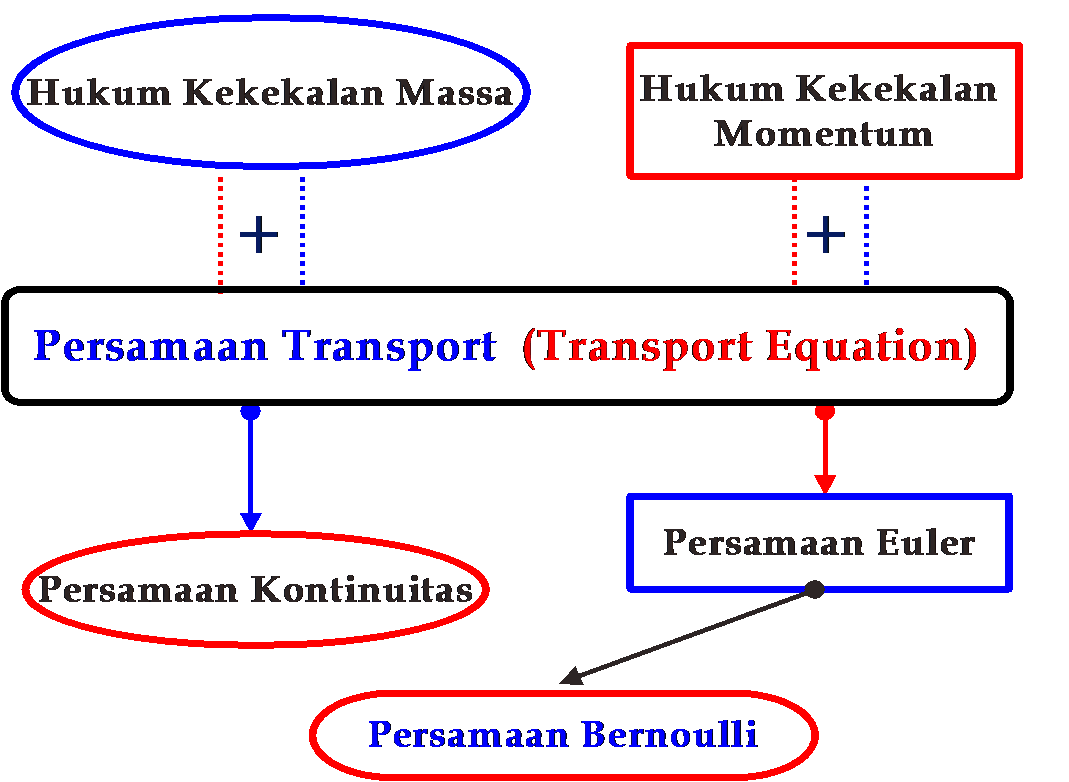
\includegraphics[scale = 4]{bagan.png}
\end{center}
\end{figure}

% Bab 3
\chapter{Teori Pembangkit Gelombang Dua Dimensi}

Kita akan membandingkan dua teori pembangkit gelombang yang telah diselidiki
dan dibuat model matematisnya. Bagian yang pertama adalah teori yang
disederhanakan yang berangkat dari ide dasar berkenaan volume air yang
dipindahkan oleh pembangkit gelombang tipe \textit{'flap'} pada sebuah
tangki atau kolam air yang cukup panjang (\textit{towing tank}). Kemudian,
bagian yang kedua, akan diulas mengenai teori yang lebih terperinci yang
dihasilkan oleh pembangkit gelombang tipe {\itshape'flap'} di salah satu
ujung \textit{towing tank} tadi. Dari hasil kedua teori ini, kita akan
mengamati perbandingan antara amplitudo gelombang yang dihasilkan $H$ dengan
besarnya simpangan maksimum pembangkit gelombang $S$ (\textit{stroke}).

Di dalam pembahasan tugas akhir ini, teori yang lebih terperinci tersebut
didasarkan atas {\itshape'teori gelombang linear'\ } yang dibahas dan
dikembangkan oleh Airy\footnote[1]{\textbf{Airy, Sir George Biddel (1801-92).%
}$\;$ Matematikawan dan fisikawan Inggris, yang menjadi astronom
kerajaan (Astronomer Royal) selama 46 tahun; dia memberikan
sumbangan pada teori-teori cahaya dan, tentulah, pada astronomi,
tetapi juga pada gravitasi, kemagnetan dan suara, sebagaimana
halnya pada perambatan gelombang secara umum dan pada teori
pasang-surut air pada khususnya. \cite{jrs}} sekitar 160 tahun
yang lalu, dalam menganalisis perilaku gelombang air laut.
\cite{aph}

% Section 3.1
\section{Teori Pembangkit Gelombang yang\\ Disederhanakan}

Di dalam air dangkal, teori sederhana untuk profil perambatan gelombang yang
dihasilkan oleh suatu pembangkit gelombang pertama kali dikembangkan oleh
Galvin pada tahun 1964, yang bernalar bahwa air yang dipindahkan oleh suatu
pembangkit gelombang seharusnya sama dengan volume puncak dari bentuk
gelombang yang merambat. Pertimbangkan sebuah pembangkit gelombang tipe flap
yang ujung bawahnya terikat dan mempunyai simpangan maksimum \textit{stroke}
$S$. Kedalaman air dalam \textit{towing tank} adalah $h$. Volume air yang
dipindahkan oleh simpangan flap adalah $\displaystyle\frac{1}{2}\,S\,h$.
Lihat Gambar 3.1. Volume air dalam suatu puncak gelombang adalah $%
\displaystyle\int_{0}^{\frac{1}{2}\,L}\frac{1}{2}\,H\sin \:k\,x\:dx$ dengan $k=%
\displaystyle\frac{2\,\pi }{L}$ adalah bilangan gelombang. Dengan demikian,
\begin{eqnarray}
\displaystyle\int\limits_{0}^{\frac{1}{2}\,L}\frac{1}{2}\:H\:\sin
\:(k\,x)\:dx
&=&\displaystyle\int_{0}^{\frac{1}{2}\,L}\frac{1}{2}\:H\:\sin \Bigg(\frac{%
2\,\pi }{L}x\Bigg)\:dx \\ \vspace{0.5cm}
&=&\displaystyle\frac{H\,L}{2\,\pi } \\ \vspace{0.5cm}
&=&\displaystyle\frac{H}{k}
\end{eqnarray}
Dengan menyamakan kedua volume,
\[
\frac{1}{2}\,S\,h=\frac{H}{k}=H\,\frac{L}{2\,\pi }=\frac{H}{2}\Bigg(\frac{L}{%
2}\Bigg)\:\frac{2}{\pi }
\]
dengan $\displaystyle\frac{2}{\pi }$ adalah faktor yang menyatakan
perbandingan antara luas daerah yang dibentuk oleh profil gelombang dengan
persegipanjang yang melingkupinya (yang disebut juga dengan istilah {\textbf{%
faktor luas.}}) Dari persamaan $\displaystyle\frac{1}{2}\,S\,h=\frac{H}{k}$,
kita bisa mengetahui besarnya perbandingan ketinggian gelombang $H$ dengan
simpangan $S$, yaitu
\[
\frac{H}{S}=\frac{1}{2}\,k\,h.
\]
Hubungan ini berlaku hanya untuk daerah air dangkal, yakni $\displaystyle k\,h<\frac{1}{10}\pi$.
%\newpage
\begin{figure}[h]
\begin{center}
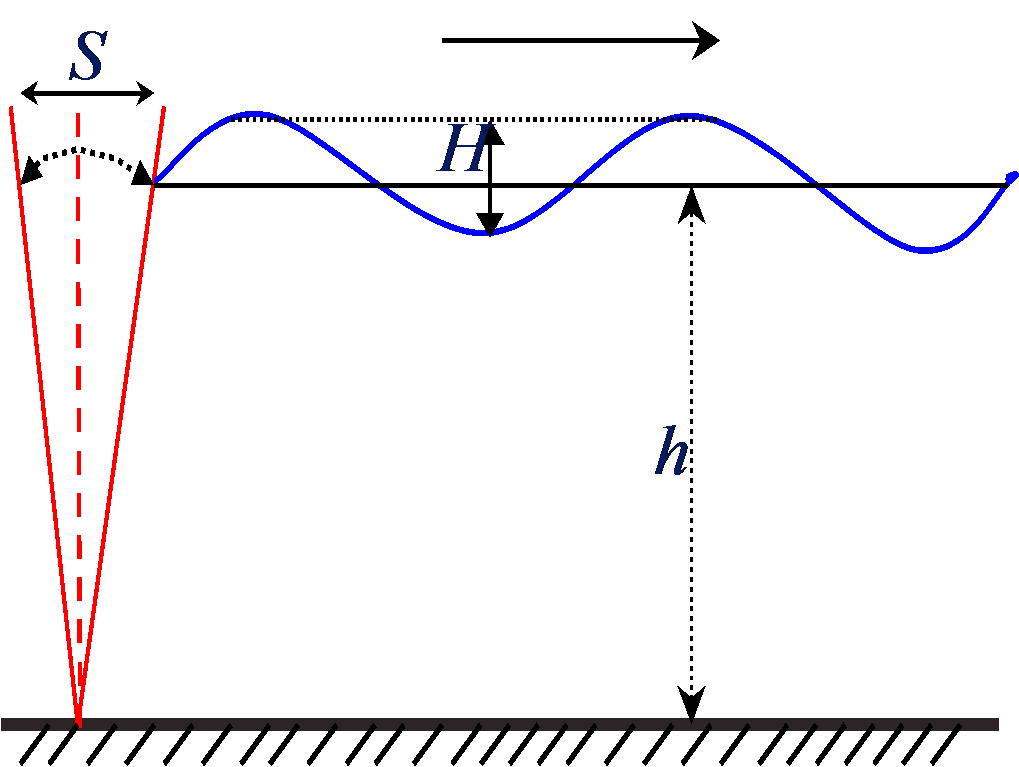
\includegraphics[scale = 3]{skema.png}
\end{center}
\caption{Skema pembangkit gelombang tipe flap.}
\end{figure}

% Section 3.2
\section{Teori Pembangkit Gelombang Linear}

Berdasarkan asumsi bahwa air adalah fluida yang tak termampatkan (\textit{%
incompressible}), maka dari hasil di sub-bab \ref{kontinuitas}, persamaan (%
\ref{vpk}), kita telah mempunyai $\nabla\cdot\mathbf{u}=0$. Selain itu,
asumsi lain yang digunakan adalah tidak adanya pusaran air (\textit{whirpool}%
), dengan kata lain, aliran air tak berputar
(\textit{irrotational}). Berdasarkan asumsi ini, dari penjelasan
di sub-bab \ref{bernoulli}, kita telah mendapatkan
$\mathbf{u}=\nabla\,\phi$. Apabila kedua persamaan ini
digabungkan, maka kita peroleh
$\nabla\cdot\nabla\,\phi=\nabla^{2}\phi=0$. Persamaan ini dikenal
dengan persamaan Laplace,\footnote[1]{\textbf{Laplace, Marquis
Pierre Simon de (1749-1827).}$\;$ Matematika-fisikawan Perancis
yang memberikan sumbangan pada studi mengenai celestial mekanika
dan, pada khususnya, menjelaskan orbit planet Yupiter dan
Saturnus; dia mengembangkan ide dalam menggunakan fungsi potensial
dan fungsi ortogonal, serta memperkenalkan transformasi
integralnya; dia juga memainkan peranan penting dalam perkembangan
teori peluang.} yang merupakan persamaan diferensial pengatur
(\textit{governing differential equation}) untuk potensial
kecepatan $\phi$. Dalam koordinat kartesius untuk dua dimensi
\textbf{---} arah horizontal (sumbu $x$) dan arah vertikal (sumbu
$z$) \textbf{---} persamaan Laplace dapat dituliskan sebagai
\begin{eqnarray}
\nabla^2\phi = \frac{\partial^2\phi}{\partial x^2}+\frac{\partial^2\phi}{%
\partial z^2}=0,
\end{eqnarray}
dan persamaan ini berlaku pada daerah $-h \,\leq\, z \, \leq\, \eta(x,\,t)$,
\quad $0 \,\leq\, x\, \leq \,\infty$.

Masalah nilai batas yang terkait di sini adalah persoalan nilai batas untuk
perambatan gelombang dua dimensi dalam suatu fluida ideal. Kita akan
memecahkan persamaan tersebut dengan beberapa syarat batas yang sesuai
dengan kondisi \textit{towing tank}. Setidaknya, kita memiliki tiga buah
kondisi syarat batas yang akan membantu kita untuk memecahkan persamaan
penuntun di atas. Berikut ini adalah syarat batas yang berkaitan dengan
kondisi \textit{towing tank}.

% Subsection 3.2.1
\subsection{Syarat batas lateral di pembangkit gelombang\\ (\textit{pseudo-boundary})}

Misal fungsi yang menggambarkan pergeseran horizontal pada permukaan
pembangkit gelombang adalah
\begin{eqnarray}
F(x,\,z,\,t) = x - \frac{1}{2}\,S(z)\:\sin \:\omega\, t = 0,
\end{eqnarray}
maka dengan melakukan diferensial total pada $F(x,\,z,\,t)$, kita peroleh
\begin{equation}
\frac{DF}{Dt} = \frac{\partial F}{\partial t} + \frac{\partial F}{\partial x}
\frac{dx}{dt} + \frac{\partial F}{\partial z} \frac{dz}{dt}
\end{equation}
\begin{equation}
0 = -\frac{1}{2}\:\omega\: S(z)\: \cos\: \omega\, t + v - \frac{1}{2}\,w\:
\frac{dS(z)}{dz}\: \sin\: \omega\, t
\end{equation}
\begin{equation}
v - \frac{1}{2}\:w\: \frac{dS(z)}{dz}\: \sin\: \omega\, t = \frac{1}{2}%
\:\omega\: S(z)\: \cos\: \omega\, t \quad \textmd{pada}
\;F(x,\,z,\,t)=0
\end{equation}
dengan $v$ dan $w$ masing-masing adalah komponen kecepatan pada arah $x$ dan
$z$. (Ingat bahwa \textbf{u} = (v,w) adalah vektor kecepatan dua dimensi.)
Atau, persamaan ini juga dapat dituliskan sebagai
\begin{equation}
\phi_{x}=\frac{1}{2}\:\Bigg(\phi_{z}\:S\,^{\prime}(z)\:\sin\: \omega\,
t+\omega\: S(z)\:\cos\: \omega\, t\Bigg).
\end{equation}

Untuk pergeseran $S(z)$ yang cukup kecil dan kecepatan yang juga
kecil, kita dapat melinearkan persamaan tersebut dengan
mengabaikan suku kedua di ruas kiri. Seperti yang akan dilakukan
pada permukaan bebas, akan lebih tepat apabila kita mengungkapkan
syarat pada batas lateral yang bergerak dalam suku-suku yang
dievaluasi di posisi rata-ratanya, yakni pada $x = 0.$ Untuk
melakukan hal ini, kita ekspansikan syarat tersebut dalam deret
Taylor terpotong (lebih spesifik, deret Maclaurin terpotong).
\[
\displaystyle\left.\Bigg(\phi_{x}-\frac{1}{2}\,\omega\,S(z)\,\cos \omega\,t%
\Bigg)\right|_{x=\frac{1}{2}\,S(z)\,\sin\,\omega\,t} =\left.\Bigg(\phi_{x}-%
\frac{1}{2}\,\omega\,S(z)\,\cos\,\omega\, t\Bigg)\right|_{x=0}
\]
\begin{equation}
\displaystyle +\frac{1}{2}\,S(z)\,\sin\,\omega\,t\: \frac{\partial}{\partial
x}\left.\Bigg(\phi_{x}-\frac{1}{2}\,\omega\,S(z)\,\cos\,\omega\, t\Bigg)%
\right|_{x=0} + \dots.
\end{equation}
Jelaslah, hanya suku pertama dari ekspansi di atas yang linear terhadap $%
\phi_{x}$ dan S(z), sedangkan suku-suku yang lain dapat dibuang karena
diasumsikan sangat kecil. Dengan demikian, syarat batas lateral akhir
sebagai akibat dari proses linearisasi adalah persamaan
\begin{equation}
u(0,\,z,\,t)=\phi_{x}=\frac{1}{2}\;\omega\; S(z)\;\cos(\omega t).
\end{equation}

% Subsection 3.2.2
\subsection{Syarat batas di dasar \textit{towing tank} (persyaratan
kinematika)}

Karena tidak ada aliran air yang menembus ke dasar \textit{towing tank},
maka kecepatan fluida pada arah vertikal adalah sama dengan nol, yakni
\begin{equation}
\phi_{z} = \frac{\partial\phi}{\partial z} = 0, \quad
\textmd{pada} \quad z = -h.
\end{equation}

% Subsection 3.2.3
\subsection{Syarat batas di permukaan air}

\begin{itemize}
\item  \textbf{Syarat batas kinematika permukaan bebas}
\end{itemize}

Pada setiap batas, apakah ia bebas, seperti pada permukaan air,
ataupun tidak bebas (\textit{fixed}), seperti pada dasar kolam,
beberapa persyaratan fisis haruslah dipenuhi oleh kecepatan
fluida. Di bawah pengaruh gaya, batas ini bisa saja mengalami
perubahan bentuk (deformasi). Semua persyaratan ini yang bekerja
pada kinematika partikel air disebut dengan \textit{syarat batas
kinematika} (\textit{kinematics boundary conditions}). Pada setiap
permukaan fluida atau perbatasan fluida (\textit{interface}),
jelaslah bahwa tidak akan terdapat aliran yang melewati
\textit{interface}, jika tidak demikian, maka tak terdapat
\textit{interface}. Hal seperti ini sangatlah jelas dalam kasus
permukaan tetap kedap air (\textit{impermeable fixed surface})
seperti suatu lembar timbunan dinding laut (\textit{sheet pile
seawall}).\cite{drg}

Misalkan fungsi yang menggambarkan permukaan air adalah
\begin{equation}
\displaystyle G(x,\,z,\,t) = z \,-\, \eta\,(x,\,t) = 0,
\end{equation}
dengan $\eta(x,\,t)$ adalah ketinggian gelombang, yakni jarak suatu titik
pada permukaan gelombang dari permukaan bebas rata-rata atau sering dikenal
dengan istilah \textit{elevasi permukaan air.} Maka, diferensial total
persamaan di atas akan memberikan
\begin{equation}
\frac{DG}{Dt} = \frac{\partial G}{\partial t} + \frac{\partial G}{\partial x}%
\; \frac{dx}{dt} + \frac{\partial G}{\partial z}\; \frac{dz}{dt}
\end{equation}
\begin{equation}
0 = -\frac{\partial \eta}{\partial t} + \Bigg(-\frac{\partial \eta}{\partial
x}\Bigg)\:v + w
\end{equation}
atau
\begin{equation}
\eta_{t} = w - v\,\eta_{x}  \label{eta}
\end{equation}
Karena $\mathbf{u}=(v,\,w)= (\phi_{x},\phi_{z})=\nabla\phi$, maka persamaan (%
\ref{eta}) dapat dituliskan menjadi
\begin{equation}
\eta_{t} = \phi_{z} - \phi_{x}\,\eta_{x}.
\end{equation}

Definisikan $\varphi(x,\,t)= \left.\phi(x,\,z,\,t)\right|_{z=\eta(x,\,t)} =
\phi(x,\,\eta(x,\,t),\,t)$, dengan melakukan diferensiasi terhadap $x$ kita
sekarang mempunyai $\displaystyle\frac{\partial\varphi}{\partial x} = \frac{%
\partial\phi}{\partial x} + \frac{\partial\phi}{\partial\eta}\:\frac{%
\partial\eta}{\partial x}$. Kita notasikan $\displaystyle \frac{\partial \phi%
}{\partial \eta} = \gamma$. Dengan demikian, persamaan tersebut menjadi $%
\varphi_{x} = \phi_{x} + \gamma\,\eta_{x}.$ Dengan mensubstitusi $%
\displaystyle\phi_{\eta}=\frac{\partial \phi}{\partial \eta}=\gamma$ dan $%
\phi_{x} = \varphi_{x} - \gamma\,\eta_{x}$ pada persamaan di atas, kita
dapatkan persamaan
\begin{equation}
\eta_{t} = \gamma - (\varphi_{x} - \gamma\, \eta_{x})\,\eta_{x} = \gamma -
\varphi_{x}\,\eta_{x} + \gamma\, \eta_{x}^2
\end{equation}
\begin{equation}
\eta_{t} = (1 + \eta_{x}^2)\,\gamma - \varphi_{x}\,\eta_{x}.
\end{equation}
Ini adalah syarat batas kinematika permukaan bebas, yaitu kondisi yang
menyatakan fakta bahwa tidak ada partikel fluida yang dapat melewati
permukaan bebas.

\begin{itemize}
\item  \textbf{Syarat batas dinamika permukaan bebas}
\end{itemize}

Permukaan air yang "bebas", seperti pada perbatasan
(\textit{interface}) udara dan air, tidak dapat menunjang
perbedaan dalam tekanan sepanjang perbatasan dan dengan demikian
harus merespon untuk memperoleh tekanan yang seragam. Syarat
batas dinamika menggambarkan distribusi tekanan yang bekerja pada
batas yang berupa permukaan bebas dan interface.

Dari persamaan Bernoulli untuk aliran tak tunak (\textit{unsteady}), kita
telah mempunyai persamaan $\displaystyle\frac{\partial \mathbf{u}}{\partial t%
}+\nabla\Bigg(\frac{p}{\rho}+g\,z+\frac{1}{2}\mid\mathbf{u}\mid^2\Bigg)=0.$
Dengan mengasumsikan bahwa tekanan atmosfer bebas di atas lapisan air
dibatasi hanya pada permukaan bebas, persamaan di atas dapat dituliskan
menjadi
\begin{equation}
\frac{\partial {\phi}}{\partial t}+ g\,\eta+\frac{1}{2}\mid\nabla\phi%
\mid^2=0, \quad \textmd{di} \quad z =\eta(x,\,t).  \label{bernou}
\end{equation}

Sebelumnya, kita hitung dahulu $\displaystyle \frac{1}{2}\mid
\nabla\phi\mid^2$ agar diketahui representasi dalam bentuk turunan
parsialnya. Kita tahu bahwa
\begin{eqnarray}
\frac{1}{2}\mid\nabla\phi\mid^2 &=& \frac{1}{2}\,\bigg(\nabla\phi\cdot\nabla%
\phi\bigg) =\frac{1}{2}\,\bigg[\,\bigg(\phi_{x},\,\phi_{z}\bigg)\cdot \bigg(%
\phi_{x},\,\phi_{z}\bigg)\,\bigg]  \nonumber \\
&=&\frac{1}{2}\,\bigg(\phi_{x}^2+\phi_{z}^2\bigg) =\frac{1}{2}\,\bigg(%
\phi_{x}^2+\gamma^2\bigg).
\end{eqnarray}
Dengan melakukan substitusi $\phi_{x}=\varphi_{x}-\gamma\,\eta_{x}$ pada
persamaan tersebut, kita sampai pada
\begin{eqnarray}
\frac{1}{2}\mid\nabla\phi\mid^2 &=& \frac{1}{2}\,\bigg[\,\bigg(\varphi_{x}-
\gamma\,\eta_{x}\bigg)^2+\gamma^2\bigg]  \nonumber \\
&=&\frac{1}{2}\,\bigg(\varphi_{x}^2-2\gamma\,\varphi_{x}\,\eta_{x}+
\gamma^2\,\eta_{x}^2+\gamma^2\bigg)
\end{eqnarray}
Jadi, $\displaystyle \frac{1}{2}\mid\nabla\phi\mid^2 = \frac{1}{2}%
\,\varphi_{x}^2 - \gamma\,\varphi_{x}\,\eta_{x} + \frac{1}{2}\,\bigg(%
1+\eta_{x}^2\bigg)\,\gamma^2$.\newline

Dari $\varphi(x,\,t)=\phi(x,\,\eta(x,\,t),\,t)$, diferensiasi parsial
terhadap t memberikan $\displaystyle\frac{\partial\varphi}{\partial t} =
\frac{\partial\phi}{\partial t} + \frac{\partial\phi}{\partial\eta}\frac{%
\partial\eta}{\partial t}$ \quad $\Longrightarrow \varphi_{t} = \phi_{t} +
\gamma\,\eta_{t}$ $\Longrightarrow \phi_{t} = \varphi_{t} - \gamma\,\eta_{t}$%
.

Dengan demikian, substitusi pada persamaan Bernoulli (\ref{bernou}) akan
menghasilkan
\begin{equation}
\varphi_{t} - \gamma\,\eta_{t} + \frac{1}{2}\,\varphi_{x}^2 -
\gamma\,\varphi_{x}\,\eta_{x} + \frac{1}{2}\,\bigg(1+\eta_{x}^2\bigg)%
\,\gamma^2 + g\,\eta=0.
\end{equation}
Untuk memperoleh bentuk yang lebih sederhana, kita substitusi $\eta_{t} = %
\bigg(1 + \eta_{x}^2\bigg)\,\gamma - \varphi_{x}\,\eta_{x}$ yang telah
diperoleh dari syarat batas kinematika. Akibatnya,
\begin{equation}
\varphi_{t} - \gamma\,\bigg[\,\bigg(1 + \eta_{x}^2\bigg)\,\gamma -
\varphi_{x}\,\eta_{x}\bigg] + \frac{1}{2}\,\varphi_{x}^2 -
\gamma\,\varphi_{x}\,\eta_{x} + \frac{1}{2}\,\bigg(1+\eta_{x}^2\bigg)%
\,\gamma^2 + g\,\eta=0,
\end{equation}
\begin{equation}
\varphi_{t} - \bigg(1 + \eta_{x}^2\bigg)\,\gamma^2 +
\varphi_{x}\,\eta_{x}\,\gamma + \frac{1}{2}\,\varphi_{x}^2 -
\gamma\,\varphi_{x}\,\eta_{x} + \frac{1}{2}\,\bigg(1+\eta_{x}^2\bigg)%
\,\gamma^2 + g\,\eta=0,
\end{equation}
\begin{equation}
\varphi_{t} - \frac{1}{2}\,\bigg(1+\eta_{x}^2\bigg)\,\gamma^2 + \frac{1}{2}%
\,\varphi_{x}^2 + g\,\eta=0.
\end{equation}
Akhirnya diperoleh, $\displaystyle\varphi_{t}=\frac{1}{2}\,\bigg(1+\eta_{x}^2%
\bigg)\,\gamma^2 -\frac{1}{2}\,\varphi_{x}^2 - g\,\eta$. Persamaan inilah
yang dikenal dengan syarat batas dinamika permukaan bebas.
\begin{figure}[h]
\begin{center}
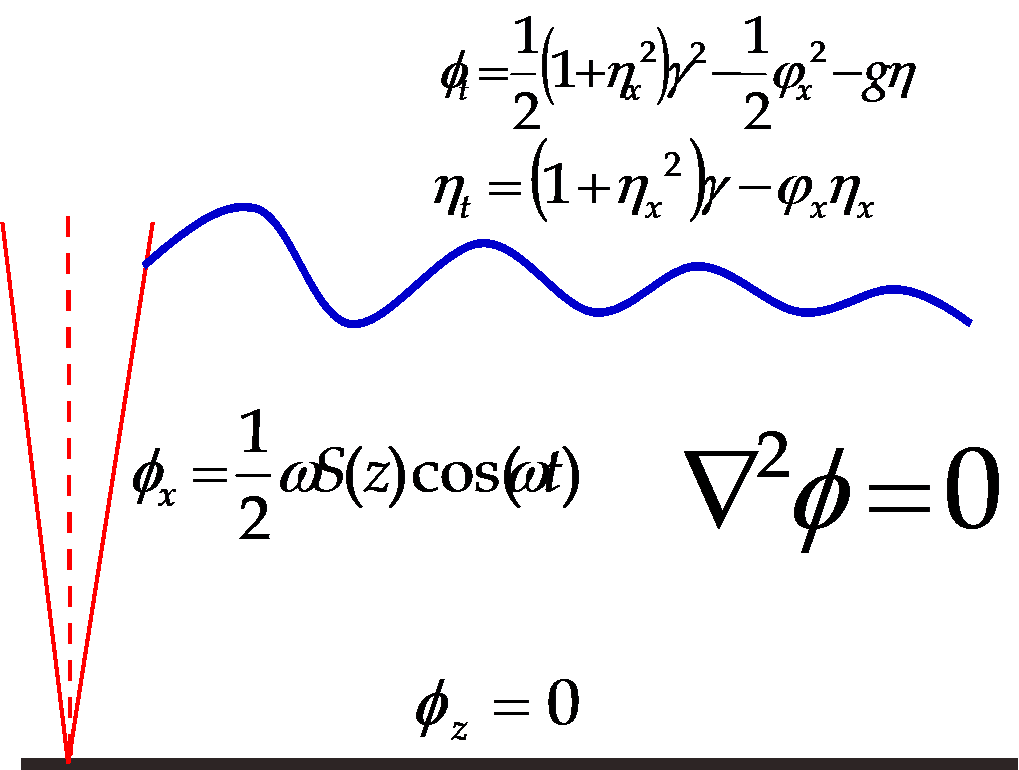
\includegraphics[scale = 3]{governing.png}
\end{center}
\caption{Skema pembangkit gelombang dengan persamaan pengatur dan syarat-syarat batasnya.}
\end{figure}

Untuk air dangkal, kita lebih tertarik untuk mempelajari dan menggunakan
bentuk terlinearisasi dari syarat batas kinematika dan syarat batas dinamika
permukaan bebas agar lebih memudahkan dalam menyelesaikan persamaan
diferensial pengatur dengan syarat-syarat batas yang telah ditentukan.

Tinjau kembali persamaan (\ref{eta}) sebagai syarat batas kinematika
permukaan bebas,
\begin{equation}
\frac{\partial \eta}{\partial t}= \left.(w)\right|_{z=\eta}- \frac{\partial
\eta}{\partial x}\,\left.(v)\right|_{z=\eta}
\end{equation}
atau
\begin{equation}
\frac{\partial \eta}{\partial t}= \left.\Bigg(\frac{\partial \phi}{\partial z%
}\Bigg)\right|_{z=\eta} - \frac{\partial \eta}{\partial x}\, \left.\Bigg(%
\frac{\partial \phi}{\partial x}\Bigg)\right|_{z=\eta}
\end{equation}
Dengan mengabaikan suku-suku non-linear-nya, kita miliki bentuk yang lebih
sederhana dari syarat batas kinematika, yakni
\begin{equation}
\left.\Bigg(\frac{\partial \phi}{\partial z} \Bigg)\right|_{z=0}=\frac{%
\partial\eta}{\partial t}.
\end{equation}

Dengan cara serupa, kita juga mempunyai bentuk yang lebih sederhana dari
syarat batas dinamika permukaan bebas, yakni
\begin{equation}
\left. \Bigg(\frac{\partial \phi }{\partial t}\Bigg)\right| _{z=0}=-g\,\eta .
\label{permukaan}
\end{equation}

Skema pembangkit gelombang dengan \textit{governing equation} dan
beberapa syarat batas dapat dilihat pada Gambar 3.2.

% Section 3.3
\section{Solusi \textit{Governing Differential Equation}}

Berikut ini adalah solusi umum potensial kecepatan
\[
\phi(x,\,z,\,t)=A_{p}\:\cosh \,k_{p}\,(h+z)\:\sin\,(k_{p}\,x-\omega\,
t)+(A\,x+B)
\]
\begin{equation}
+ C\:e^{-k_{s}\,x}\:\cos k_{s}\,(h+z)\:\cos \,\omega\, t.
\end{equation}
Untuk permasalahan pembangkit gelombang, koefisien A di atas haruslah sama
dengan nol karena tidak ada aliran seragam yang mungkin melalui pembangkit
gelombang dan koefisien B di atas juga dapat diset menjadi nol juga tanpa
mempengaruhi medan kecepatan. Suku-suku sisanya haruslah memenuhi dua syarat
batas permukaan bebas yang terlinearisasi. Biasanya akan lebih bermanfaat
apabila menggabungkan kedua syarat batas tersebut menjadi bentuk yang lebih
sederhana.\newline
Dengan menurunkan $\phi$ terhadap t, kita peroleh
\[
\frac{\partial\phi}{\partial t}=-\,\omega\, A_{p}\:\cosh\,
k_{p}\,(h+z)\:\cos\,(k_{p}\,x-\omega\, t)
\]
\begin{equation}
-\,\omega\, C\,e^{-k_{s}\,x}\:\cos k_{s}\,(h+z)\:\sin \omega\, t.
\end{equation}
Turunan kedua $\phi$ terhadap t menghasilkan
\begin{eqnarray}
\frac{\partial^2\phi}{\partial t^2} &=& -\,\omega^2\, A_{p}\:\cosh\,
k_{p}\,(h+z)\:\sin\,(k_{p}\,x-\omega\, t)  \nonumber \\
& & -\, \omega^2\, C\,e^{-k_{s}\,x}\:\cos k_{s}\,(h+z)\:\cos\, \omega\, t
\nonumber \\
&=& -\,\omega^2\,\phi.
\end{eqnarray}
Tetapi dari syarat batas dinamika dan kinematika permukaan bebas kita punya
\begin{equation}
\frac{\partial \eta}{\partial t}=-\,\frac{1}{g}\,\frac{\partial^2\phi}{%
\partial t^2}= -\,\frac{\omega^2}{g}\,\phi = -\,\frac{\partial \phi}{%
\partial z}, \quad \textmd{pada} \quad z = 0,
\end{equation}
atau
\begin{equation}
\frac{\partial \phi}{\partial z}-\frac{\omega^2}{g}\,\phi=0, \quad \textmd{pada} \quad z = 0.
\end{equation}
Dengan mensubstitusi solusi yang telah kita asumsikan pada persamaaan ini,
maka dihasilkan
\begin{equation}
\omega^2 = g\,k_{p}\: \tanh\: k_{p}\,h  \label{progresif}
\end{equation}
dan
\begin{equation}
\omega^2 = -g\,k_{s} \:\tan\: k_{s}\,h.  \label{berdiri}
\end{equation}
Persamaan yang pertama adalah relasi dispersi untuk gelombang progresif.
Dengan menuliskan kembali persamaan tersebut menjadi
\begin{equation}
\frac{\omega^2\,h}{g\,k_{p}\,h}= \tanh\:k_{p}\,h
\end{equation}
dan mengeplot tiap suku terhadap $k_{p}\,h$ untuk nilai $\displaystyle \frac{%
\omega^2\,h}{g}$ tertentu, maka kita bisa melihat solusi untuk relasi
dispersi tersebut seperti diperlihatkan pada Gambar \ref{gambar2}.
\begin{figure}[h]
\begin{center}
%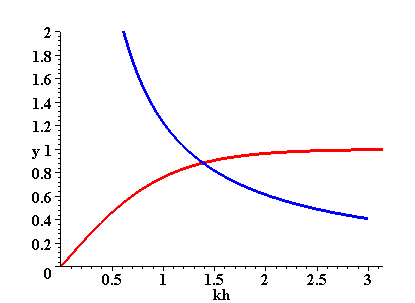
\includegraphics[natheight=228.125pt, natwidth=312.4375pt, height=231.375pt, width=316.125pt ]{progresif.png}\\[0pt]
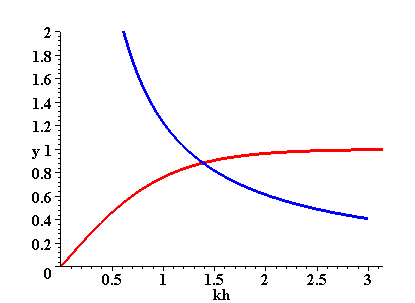
\includegraphics[scale = 0.8]{progresif.png}
\end{center}
\par
{Grafik ini mengilustrasikan akar tunggal $k_{p}\,h$. Label sumbu horizontal
\textbf{kh} memaksudkan $k_{p}\,h$.}
\caption{Grafik relasi dispersi gelombang progresif}
\label{gambar2}
\end{figure}

Persamaan (\ref{berdiri}), yang mengaitkan $k_{s}$ dengan frekuensi
pembangkit gelombang, menentukan bilangan gelombang untuk gelombang berdiri
dengan amplitudo yang berkurang secara eksponensial seraya menjauh dari
pembangkit gelombang. Dengan menuliskan kembali persamaan tersebut sebagai
\begin{equation}
\frac{\omega^2\,h}{g\,k_{s}\,h}=-\tan\:k_{s}\,h,
\end{equation}
maka dengan mengeplot grafiknya kita bisa melihat bahwa ia mempunyai tak
hingga banyaknya penyelesaian. Penyelesaian persamaan ini dapat dilihat
dalam bentuk grafik relasi dispersi, seperti tampak pada Gambar~\ref{gambar3}.
\begin{figure}[h]
\caption{Grafik relasi dispersi gelombang berdiri} 				\label{gambar3}
\begin{center}
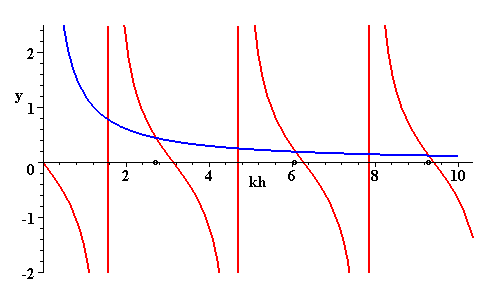
\includegraphics[scale = 0.8]{standing.png}
\end{center}
\par
{Grafik ini mengilustrasikan terdapat tak hingga banyaknya akar majemuk $k_{s}(n)\,h$. Label sumbu horizontal \textbf{kh} memaksudkan $k_{s}\,h$.}
\end{figure}

Setiap penyelesaian akan dinyatakan dengan $k_{s}(n)$, dengan $n$ bilangan
asli. Bentuk akhir dari potensial kecepatan adalah
\[
\phi(x,\,z,\,t)=A_{p}\:\cosh\,k_{p}\,(h+z)\:\sin\,(k_{p}\,x-\omega\,t)
\]
\begin{equation}
+ \mathop {\sum}_{n=1}^{\infty} C_{n}\:e^{-k_{s}(n)\,x}\:\cos\,
k_{s}(n)\,(h+z)\:\cos\, \omega \,t.  \label{lastpotensial}
\end{equation}
Suku pertama menyatakan gelombang progresif yang dihasilkan oleh pembangkit
gelombang, sedangkan suku deret menyatakan gelombang berdiri yang semakin
meluruh seraya menjauh dari pembangkit gelombang.

Untuk memperoleh solusi gelombang yang lengkap, kita harus menentukan $A_{p}$
dan $C_{n}$. Nilai-nilai ini diperoleh dengan bantuan syarat batas lateral
di pembangkit gelombang, yakni
\begin{equation}
u(0,\,z,\,t)=\left.\Bigg(\frac{\partial \phi}{\partial x}\Bigg)\right|_{x=0}
= \frac{1}{2}\:\omega\,S(z)\:\cos\,\omega\,t
\end{equation}
Dengan menurunkan potensial kecepatan terhadap $x$ dan mengevaluasinya di $%
x=0$, kita memperoleh
\[
\frac{1}{2}\:\omega\,S(z)\:\cos\,\omega\,t =
A_{p}\,k_{p}\:\cosh\,k_{p}\,(h+z)\:\cos\,\omega\,t
\]
\begin{equation}
-\mathop {\sum}_{n=1}^{\infty} C_{n}\,k_{s}(n)\:\cos\,
k_{s}(n)\,(h+z)\:\cos\, \omega \,t,
\end{equation}
atau
\begin{equation}
\frac{1}{2}\:\omega\,S(z) = A_{p}\,k_{p}\:\cosh\,k_{p}\,(h+z)-\mathop {\sum}%
_{n=1}^{\infty} C_{n}\,k_{s}(n)\:\cos\, k_{s}(n)\,(h+z).  \label{fourier}
\end{equation}
Sekarang kita mempunyai sebuah fungsi $z$ yang sama dengan suatu deret
fungsi-fungsi trigonometri dari $z$ di ruas kanan, situasi yang mirip dengan
deret Fourier. Kita punya fakta bahwa himpunan fungsi-fungsi $\displaystyle%
\bigg\{\cosh\,k_{p}\,(h+z),\; \cos\, [k_{s}(n)\,(h+z)]\bigg\}_{n=1}^{\infty}$
membentuk suatu deret harmonik lengkap fungsi-fungsi ortogonal, dan
sembarang fungsi kontinu dapat diekspansi dalam suku-suku deret tersebut.

Dengan demikian, untuk mencari $A_{p},$ kalikan persamaan di atas dengan $%
\cosh\,k_{p}\,(h+z)$ dan diintegrasikan terhadap $z$ dari $-h$ sampai $0$.
Kita sekarang mempunyai
\[
\mathop {\int}_{-h}^{0}\: \frac{1}{2}\:\omega\,S(z)\:\cosh\,k_{p}\,(h+z)%
\,dz= \mathop {\int}_{-h}^{0}\:A_{p}\,k_{p}\:\cosh\,k_{p}^2\,(h+z)\,dz
\]
\begin{equation}
-\mathop {\int}_{-h}^{0}\; \mathop {\sum}_{n=1}^{\infty}
C_{n}\,k_{s}(n)\:\cos\,k_{s}(n)\,(h+z)\:\cosh\,k_{p}\,(h+z)\,dz.
\end{equation}
Dengan menggunakan sifat keortogonalan, suku terakhir akan sama dengan nol,
dan akibatnya
\begin{equation}
A_{p}=\frac{\frac{1}{2}\:\omega\:\int_{-h}^{0}\:S(z)\:\cosh\,k_{p}\,(h+z)\,dz%
} {k_{p}\:\mathop {\int}_{-h}^{0}\:\cosh\,k_{p}^2\,(h+z)\,dz}
\end{equation}
Untuk pembangkit gelombang tipe flap, fungsi simpangan $S$ dapat
dinyatakan secara spesifik sebagai
\begin{equation}
S(z)=S\,\Bigg(1+\frac{z}{h}\Bigg).
\end{equation}
Dengan menggunakan kalkulus sederhana kita bisa menyatakan koefisien $A_{p}$
tanpa menggunakan integral, yaitu
\begin{equation}
A_{p}=\frac{2\,\omega\,S}{k_{p}^2\,h}\;\frac{k_{p}\,h\:\sinh\,k_{p}\,h
-\cosh\,k_{p}\,h+1}{\sinh\,2\,k_{p}\,h+2\,k_{p}\,h}  \label{firstconst}
\end{equation}

Dengan cara yang serupa, kita bisa mendapatkan koefisien $C(n)$ dengan
mengalikan persamaan (\ref{fourier}) dengan $\cos\,[k_{s}(n)\,(h+z)]$ dan
mengintegrasikannya terhadap $z$ dari $-h$ sampai dengan 0 (sepanjang
kedalaman). Kita dapatkan
\begin{equation}
C_{n}=\frac{-\frac{1}{2}\:\omega\:\int_{-h}^{0}\:S(z)\:\cos\,k_{s}(n)\,(h+z)%
\,dz} {k_{s}(n)\:\int_{-h}^{0}\:\cos^2\,[k_{s}(n)\,(h+z)]\,dz}
\end{equation}
atau, dengan melakukan sedikit proses integrasi kita sampai pada hasil
berikut :
\begin{equation}
C_{n}=\frac{-2\,\omega\,S}{[k_{s}(n)]^2\,h}\;\frac{[k_{s}(n)\,h]\:\sin%
\,[k_{s}(n)\,h]+ \cos\,[k_{s}(n)\,h]}{\sin\,[2\,k_{s}(n)\,h]+2\,k_{s}(n)\,h}.
\label{nextconst}
\end{equation}
Tinggi gelombang untuk gelombang progresif ditentukan dengan mengevaluasi $%
\eta$ cukup jauh dari pembangkit gelombang.
\begin{eqnarray}
\eta=-\frac{1}{g}\left.\Bigg(\frac{\partial \phi}{\partial t}\Bigg)%
\right|_{z=0} &=& \frac{A_{p}}{g}\,\omega\: \cosh\,k_{p}\,h
\:cos\,(k_{p}\,x-\omega\,t)  \nonumber \\
&=&\frac{H}{2}\:\cos\,(k_{p}\,x-\omega\,t) \quad x\gg\, h
\end{eqnarray}
Dengan mensubstitusi nilai $A_{p}$ yang telah diperoleh, kita bisa
mendapatkan perbandingan tinggi gelombang $H$ dengan besarnya stroke $S$,
yaitu
\begin{equation}
\frac{H}{S}= 4\: \Bigg(\frac{\sinh\,k_{p}\,h}{k_{p}\,h}\Bigg)\; \Bigg(\frac{%
k_{p}\,h\:\sinh\,k_{p}\,h-\cosh\,k_{p}\,h+1}{\sinh\,2\,k_{p}\,h+ 2\,k_{p}\,h}%
\Bigg).  \label{ratio}
\end{equation}
Plot grafik perbandingan $H$ dan $S$, baik untuk teori yang disederhanakan
(air dangkal) maupun yang lebih lengkap (teori pembangkit gelombang linear)
dapat dilihat pada Gambar~\ref{gambar1}.
\begin{figure}[h]
\caption{Grafik perbandingan ketinggian gelombang $H$ dengan simpangan $S$ terhadap kedalaman relatif $k_{p}\,h$.}
\label{gambar1}
\begin{center}
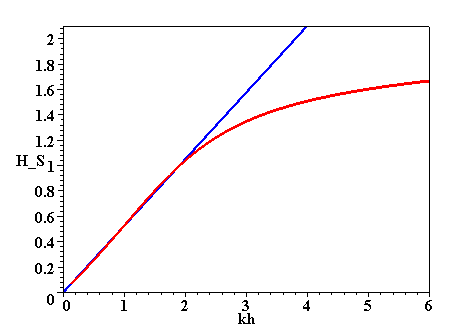
\includegraphics[scale = 0.8]{HSkh.png}
\end{center}
\par
{Label sumbu horizontal \textbf{kh} memaksudkan $k_{p}\,h$, sedangkan label sumbu vertikal \textbf{H\_S} memaksudkan $\displaystyle\frac{H}{S}$.}
\end{figure}

% Bab 4
\chapter{Simulasi Numerik}

Pada bab ini, akan dibahas beberapa hasil yang diperoleh dengan memilih
nilai-nilai besaran tertentu. Dengan bantuan perangkat lunak \textit{Maple V
Release 5}, kita bisa melihat animasi gelombang monokromatik yang dihasilkan
apabila pembangkit gelombang digerakkan dengan simpangan tertentu.

% Section 4.1
\section{Menghitung Bilangan Gelombang Progresif} 		\label{NR1}

Kita perhatikan kembali persamaan (\ref{progresif}) yang menyatakan relasi
dispersi gelombang progresif :
\begin{equation}
\omega^2 = g\,k_{p}\: \tanh\: k_{p}\,h.
\end{equation}
Untuk memperoleh nilai bilangan gelombang $k_{p}$, kita tidak dapat
menghitungnya secara eksak, sehingga digunakan metode numerik untuk
menyelesaikannya. Beberapa nilai yang diberikan adalah frekuensi sudut
monokromatik $\omega = 2$ rad/detik, tetapan percepatan gravitasi $g = 9,8 $
m/detik$^2$, dan kedalaman \textit{towing tank} $h = 3$ m. Dengan
menggunakan iterasi \textit{Newton-Raphson}, kita akan mencari nilai $k_{p}$
apabila diberikan tebakan awal $p_{0}$ dengan mencari akar persamaan $%
f(k_{p})=0$, dengan $f(k_{p}) = \omega^2 - g\,k_{p}\: \tanh\: k_{p}\,h$.
Untuk mengetahui lebih lengkap mengenai algoritma iterasi \textit{%
Newton-Raphson}, dapat dilihat di Apendiks B. Dengan memilih nilai-nilai
galat $\delta = 10^{-9}, \quad \epsilon = 10^{-9},$ dan $kecil = 10^{-9}$
juga, serta iterasi maksimum = 5000, maka dengan menggunakan tebakan awal $%
p_{0} = 0,5$ kita memperoleh hasil $k_{p} = 0,4624593666$. Lihat grafiknya
pada Gambar \ref{gambar2}.

Untuk $\omega = 1$, nilai bilangan gelombang progresif yang diperoleh adalah
$k_{p} = 0,1943823443$.

% Section 4.2
\section{Menghitung Bilangan Gelombang Berdiri} \label{NR2}

Kita perhatikan kembali persamaan (\ref{berdiri}) yang menyatakan relasi
dispersi gelombang berdiri :
\begin{equation}
\omega^2 = -g\,k_{s}\: \tan\: k_{s}\,h.
\end{equation}
Untuk memperoleh nilai bilangan gelombang $k_{s}$, kita tidak dapat
menghitungnya secara eksak, sehingga digunakan metode numerik untuk
menyelesaikannya. Beberapa nilai yang diberikan adalah frekuensi sudut
monokromatik $\omega = 2$ rad/detik, tetapan percepatan gravitasi $g = 9,8 $
m/detik$^2$, dan kedalaman \textit{towing tank} $h = 3$ m. Dengan
menggunakan iterasi \textit{Newton-Raphson}, kita akan mencari nilai $k_{s}$
apabila diberikan tebakan awal $p_{0}$ dengan mencari akar persamaan $%
g(k_{s})=0$, dengan $g(k_{s}) = \omega^2 + g\,k_{s}\: \tan\: k_{s}\,h$.
Untuk mengetahui lebih lengkap mengenai algoritma iterasi \textit{%
Newton-Raphson}, dapat dilihat kembali di Apendiks B. Nilai-nilai galat yang
dipilih adalah $\delta = 10^{-5}, \quad \epsilon = 10^{-5},$ dan $kecil =
10^{-5}$ dengan menggunakan iterasi maksimum = 10000. Karena perpotongan
grafik pada relasi dispersi menghasilkan tak hingga banyaknya titik potong,
yakni nilai-nilai bilangan gelombang berdiri, maka digunakan tebakan awal
yang bervariasi sesuai dengan kebutuhan, $p_{0} = 1, 2, 3, \cdots.$ Untuk
keperluan, kita pilih beberapa bilangan gelombang tertentu saja yang
berurutan. Akhirnya, kita memperoleh hasil\newline
$k_{s}(1)=0,9061212307;\newline
\; k_{s}(2)=2,028197863;\newline
$ $\quad k_{s}(3)=3,097926261;\newline
\quad k_{s}(4)=4,156159228;\newline
$ $\quad k_{s}(5)=5,209926525;\newline
\quad k_{s}(6)=6,261487236;\newline
$ $\quad k_{s}(7)=7,311794624;\newline
\quad k_{s}(8)=8,361321437;\newline
$ $\quad k_{s}(9)=9,410329031$.\newline
Lihat kembali grafiknya pada Gambar \ref{gambar3}.

Dengan cara yang serupa seperti di atas, yakni menggunakan tebakan awal yang
bervariasi, maka untuk $\omega = 1$ kita memperoleh beberapa nilai bilangan
gelombang berdiri seperti berikut:\newline
$k_{s}(1)=1,013758189;\newline
\; k_{s}(2)=2,078040121;\newline
\; k_{s}(3)=3,130732073;\newline
\; k_{s}(4)=4,180655871$.\newline

% Section 4.3
\section{Profil Gelombang Monokromatik}

% Subsection 4.3.1
\subsection{Dua Profil Gelombang dengan Ketinggian \textit{\textbf{H}} Berbeda}

Perhatikan kembali persamaan (\ref{lastpotensial}), persamaan potensial
kecepatan yang menggambarkan gelombang air yang dihasilkan oleh pembangkit
gelombang
\[
\phi(x,\,z,\,t)=A_{p}\:\cosh\,k_{p}\,(h+z)\:\sin\,(k_{p}\,x-\omega\,t)
\]
\begin{equation}
+ \mathop {\sum}_{n=1}^{\infty} C_{n}\:e^{-k_{s}(n)\,x}\:\cos\,
k_{s}(n)\,(h+z)\:\cos\, \omega \,t.
\end{equation}
Dengan menggunakan persamaan (\ref{firstconst}) dan persamaan (\ref{ratio}),
kita bisa menyatakan konstanta $A_{p}$ dalam $\omega$, $H$, $k_{p}$, dan $h$, yakni :
\begin{equation}
A_{p}=\frac{\omega\,H}{2\,k_{p}\:\sin\:k_{p}\,h}
\end{equation}
Dengan mensubstitusi nilai $\omega = 2$, $k_{p} = 0,4624593666$, dan $h = 3$%
, maka :

\begin{itemize}
\item  untuk $H = 0,5$, kita punya $A_{p} = 1,099621133$; dan

\item  untuk $H = 0,75$, kita punya $A_{p} = 1,649431700$.
\end{itemize}

Untuk mendapatkan simpangan maksimum $S$, kita menggunakan persamaan (\ref
{ratio}), yakni
\begin{equation}
S = \Bigg(\frac{H\,k_{p}\,h}{4\,\sinh\,k_{p}\,h}\Bigg)\; \Bigg(\frac{%
\sinh\,2\,k_{p}\,h+2\,k_{p}\,h} {k_{p}\,h\:\sinh\,k_{p}\,h-\cosh\,k_{p}\,h+1}%
\Bigg).
\end{equation}
Dengan mensubstitusi kembali nilai-nilai yang telah kita punya, akibatnya :

\begin{itemize}
\item  untuk $H = 0,5$, kita peroleh $S = 0,2908632665$; dan

\item  untuk $H = 0,75$, kita peroleh $S = 0,4362948995$.
\end{itemize}

Profil gerakan pembangkit gelombang ketika ia mencapai simpangan terjauh dapat dilihat pada Gambar~\ref{gambar4}.
\begin{figure}[h]
\begin{center}
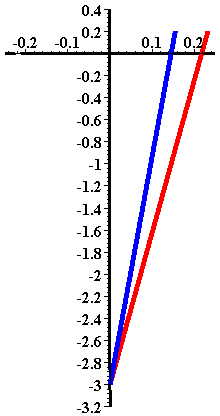
\includegraphics[scale = 0.7]{flap1.png}
\end{center}
\caption{Simpangan terjauh flap yang menghasilkan dua profil gelombang dengan ketinggian berbeda.}	\label{gambar4}
\end{figure}

Untuk mencari besarnya konstanta $C_{n}$ sebagai koefisien gelombang
berdiri, kita menggunakan persamaan (\ref{nextconst}), yaitu
\begin{equation}
C_{n}=\frac{-2\,\omega\,S}{[k_{s}(n)]^2\,h}\;\frac{[k_{s}(n)\,h]\:\sin%
\,[k_{s}(n)\,h]+ \cos\,[k_{s}(n)\,h]}{\sin\,[2\,k_{s}(n)\,h]+2\,k_{s}(n)\,h}.
\end{equation}
Nilai-nilai $k_{s}(n)$ yang telah kita punyai adalah sebanyak 4 buah, karena
untuk $n$ yang lebih besar pengaruh konstanta $C_{n}$ terhadap solusi
gelombang relatif kecil sehingga dapat diabaikan.

\begin{itemize}
\item  Untuk $S = 0,2908632665$, nilai\newline
$C_{1} = 0,08013595964$;\newline
$C_{2} = 0,00976252019$;\newline
$C_{3} = 0,001714039296$; \quad dan \newline
$C_{4} = 0,001110132786$.

\item  Untuk $S = 0,4362948995$, nilai\newline
$C_{1} = 0,1202039395$;\newline
$C_{2} = 0,01464378027$;\newline
$C_{3} = 0,002571058938$; \quad dan \newline
$C_{4} = 0,001665199177$.
\end{itemize}

Dengan menggunakan persamaan (\ref{permukaan}), yakni
\begin{equation}
\eta(x,\,t) =-\frac{1}{g}\:\left.\Bigg(\frac{\partial \phi}{\partial t}\Bigg)%
\right|_{z=0}
\end{equation}
kita dapat mencari persamaan elevasi permukaan gelombang air yang
terbentuk. Dengan bantuan perangkat lunak komputer kita juga bisa
menampilkan hasil plot permukaan. Hasil plot permukaan air dengan
dua ketinggian yang berbeda diperlihatkan pada Gambar~\ref{gambar5}.
\begin{figure}[h]
\begin{center}
%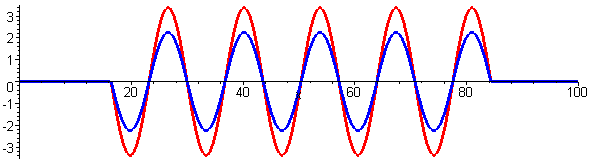
\includegraphics[natheight=122.6875pt, natwidth=445.6875pt, height=125.375pt, width=450.0625pt ]{elevasi1.png}\\[0pt]
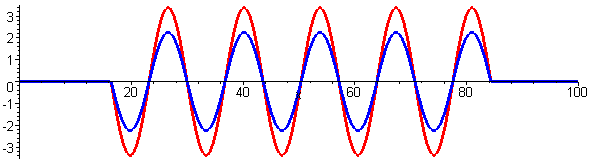
\includegraphics[scale = 0.8]{elevasi1.png}
\end{center}
\caption{Bentuk permukaan gelombang air (elevasi) yang dibentuk oleh dua gelombang dengan ketinggian yang berbeda.} 	\label{gambar5}
\end{figure}

\subsection{Dua Profil Gelombang dengan Frekuensi Sudut \textbf{$\protect \omega$} Berbeda}

Cara yang serupa seperti pada sub-bab sebelumnya diterapkan juga pada
sub-bab ini. Kedalaman \textit{towing tank} masih sama yaitu $h = 3$ m dan
profil ketinggian gelombang yang diinginkan adalah $H = 0,5$ m. Namun,
frekuensi sudut $\omega$ yang diberikan adalah masing-masing 2 dan 1. Dengan
menggunakan iterasi Newton-Raphson terhadap relasi dispersi gelombang
progresif maupun gelombang berdiri, kita bisa mendapatkan nilai $k_{p}$ dan $%
k_{s}(n)$ untuk $\omega = 1.$ Hasil-hasilnya telah diperoleh pada sub-bab
\ref{NR1} dan \ref{NR2}. Untuk lebih jelas, hasilnya dicantumkan kembali
pada sub-bab ini. Sebagai tambahan, dicantumkan juga nilai-nilai konstanta
potensial kecepatan yang berkaitan dengan nilai $\omega$, yakni $A_{p}$ dan $%
C_{n}$.

Berikut ini adalah hasil yang telah diperoleh dengan menggunakan bantuan
perangkat lunak Maple V Release 5.

\begin{description}
\item[\textbf{a.}]  Untuk $\omega = 2$

\begin{itemize}
\item[$\bullet$]  Nilai bilangan gelombang progresif $k_{p} = 0,4624593666$.

\item[$\bullet$]  Nilai-nilai bilangan gelombang berdiri \newline
$k_{s}(1)=0,9061212307;$ \quad $k_{s}(2)=2,028197863;$\newline
\quad $k_{s}(3)=3,0979262610;$ \quad $k_{s}(4)=4,156159228.$

\item[$\bullet$]  Nilai koefisien $A_{p} = 1,099621133$

\item[$\bullet$]  Besar simpangan maksimum $S = 0,2908632665$

\item[$\bullet$]  Nilai-nilai koefisien $C_{n}$ adalah \newline
$C_{1}=0,8013595964;$ \quad \quad $C_{2}=0,009762520190;$\newline
\quad $C_{3}=0,001714039296;$ \quad $C_{4}=0,001110132786.$
\end{itemize}

\item[\textbf{b.}]  Untuk $\omega = 1$

\begin{itemize}
\item[$\bullet$]  Nilai bilangan gelombang progresif $k_{p} = 0,1943823443$.

\item[$\bullet$]  Nilai-nilai bilangan gelombang berdiri \newline
$k_{s}(1)=1,013758189; \quad k_{s}(2)=2,078040121;\newline
\; k_{s}(3)=3,130732073; \quad k_{s}(4)=4,180655871$.\newline

\item[$\bullet$]  Nilai koefisien $A_{p} = 2,335633604$

\item[$\bullet$]  Besar simpangan maksimum $S = 1,140576790$

\item[$\bullet$]  Nilai-nilai koefisien $C_{n}$ adalah \newline
$\quad C_{1}=0,2125853842;$ \quad \quad $C_{2}=0,004369427564;$\newline
\quad $C_{3}=0,007018430814;$ \quad $C_{4}=0,0005323318426.$
\end{itemize}
\end{description}

Profil gerakan \textit{flap} pada saat simpangan terjauh ditunjukkan pada Gambar~\ref{gambar6}.
\begin{figure}[h]
\begin{center}
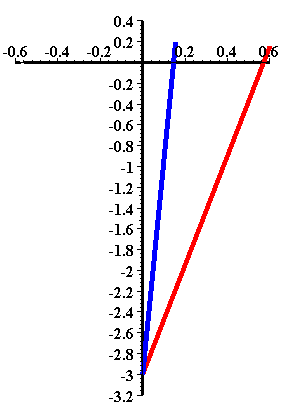
\includegraphics[scale = 0.7]{flap2.png}
\end{center}
\caption{Simpangan terjauh flap yang menghasilkan dua profil gelombang dengan frekuensi sudut berbeda.}   \label{gambar6}
\end{figure}

Profil gelombang yang dihasilkan evolusinya terhadap waktu dapat dilihat pada Gambar~\ref{gambar7} sampai dengan Gambar~\ref{gambar14}.
\begin{figure}[h]
\begin{center}
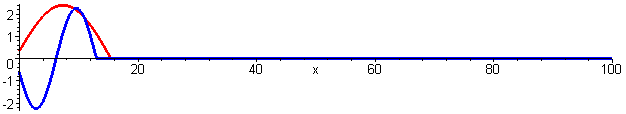
\includegraphics[scale = 0.78]{animasi3.png}
\end{center}
\caption{Grafik permukaan gelombang air pada t = 3.}   \label{gambar7}
\end{figure}

\begin{figure}[h]
\begin{center}
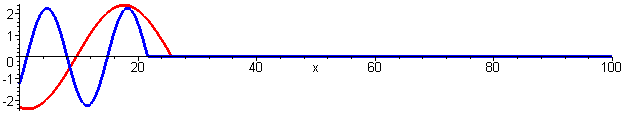
\includegraphics[scale = 0.78]{animasi5.png}
\end{center}
\caption{Grafik permukaan gelombang air pada t = 5.}   \label{gambar8}
\end{figure}

\begin{figure}[h]
\begin{center}
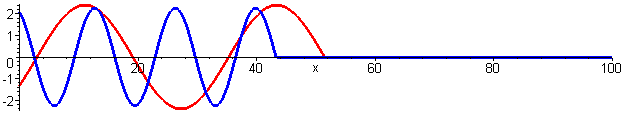
\includegraphics[scale = 0.78]{animasi10.png}
\end{center}
\caption{Grafik permukaan gelombang air pada t = 10.}  \label{gambar9}
\end{figure}

\begin{figure}[h]
\begin{center}
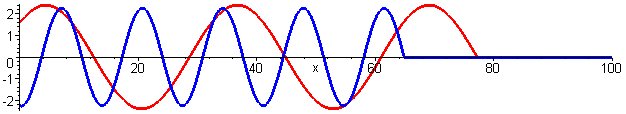
\includegraphics[scale = 0.78]{animasi15.png}
\end{center}
\caption{Grafik permukaan gelombang air pada t = 15.}  \label{gambar10}
\end{figure}

\begin{figure}[h]
\begin{center}
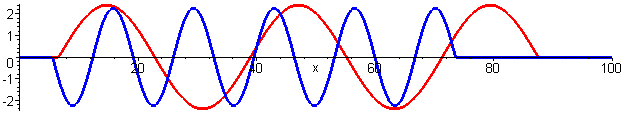
\includegraphics[scale = 0.78]{animasi17.png}
\end{center}
\caption{Grafik permukaan gelombang air pada t = 17.}   \label{gambar11}
\end{figure}

\begin{figure}[h]
\begin{center}
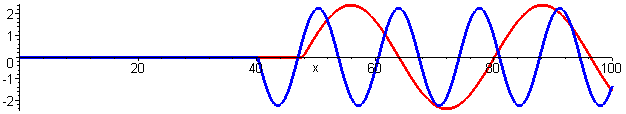
\includegraphics[scale = 0.78]{animasi25.png}
\end{center}
\caption{Grafik permukaan gelombang air pada t = 25.}   \label{gambar12}
\end{figure}

\begin{figure}[h]
\begin{center}
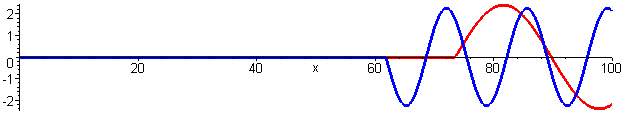
\includegraphics[scale = 0.78]{animasi30.png}
\end{center}
\caption{Grafik permukaan gelombang air pada t = 30.}   \label{gambar13}
\end{figure}

\begin{figure}[h]
\begin{center}
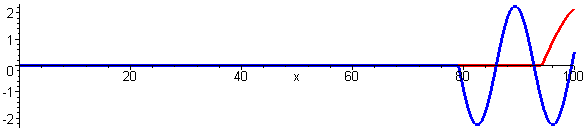
\includegraphics[scale = 0.78]{animasi34.png}
\end{center}
\caption{Grafik permukaan gelombang air pada t = 34.}   \label{gambar14}
\end{figure}

% Bab 5
\chapter{Kesimpulan dan Saran}

% Section 5.1
\section{Kesimpulan}

Berikut ini adalah beberapa kesimpulan yang diperoleh penulis setelah
mengerjakan tugas akhir mengenai pembangkit gelombang ini:

\begin{itemize}
\item[\textbf{a.}]  Asumsi fluida ideal diperlukan untuk memodelkan
permasalahan pembangkitan gelombang.

\item[\textbf{b.}]  Teori gelombang linear digunakan untuk
memperoleh pernyelesaian dari \textit{governing differential
equation} yang dihasilkan pada pemodelan pada bagian (a).

\item[\textbf{c.}]  Kaitan antara bilangan gelombang, ketinggian
gelombang, dan simpangan pembangkit gelombang diperoleh melalui
teori gelombang pada bagian (b).

\item[\textbf{d.}]  Untuk air dangkal, teori yang disederhanakan
dan teori gelombang linear memberikan hasil yang sama, sedangkan
untuk air yang lebih dalam, kedua teori tersebut memberikan hasil
yang berbeda.
\end{itemize}

% Section 5.2
\section{Saran}

Berikut ini adalah beberapa saran yang dapat dikembangkan untuk bahan tugas
akhir ataupun penelitian berikutnya :

\begin{itemize}
\item[\textbf{a.}]  Teori gelombang yang digunakan bisa menggunakan teori
gelombang non-linear dan bisa diperluas menjadi teori pembangkit gelombang
tiga dimensi.

\item[\textbf{b.}]  Tipe gelombang yang dihasilkan bisa dikembangkan menjadi
sembarang gelombang tak regular.

\item[\textbf{c.}]  Penambahan pantai (\textit{beach}) dapat
digunakan untuk menggantikan domain yang \textit{semi-infinite}.
\end{itemize}


% Appendices
\appendix

% Appendix A
\chapter{Turunan Material}

Operator
\begin{equation}
\frac{D}{Dt}=\frac{\partial}{\partial t} + \mathbf{u}\cdot \nabla  \label{op}
\end{equation}
dikenal sebagai turunan \textit{material}, turunan \textit{total},
turunan \textit{substansial}, atau turunan \textit{Lagrange}.
Secara umum, $\displaystyle \frac{D}{Dt}$ adalah suatu operator
vektor. Akibatnya, komponen-komponen $\displaystyle \frac{D}{Dt}$
yang bekerja pada vektor tidaklah sama dengan yang bekerja pada
komponen skalar suatu vektor, kecuali dalam koordinat Kartesius.
Operator turunan material dapat juga diterapkan pada besaran
skalar, seperti temperatur. Secara fisis, ini menyatakan perubahan
besaran tersebut terhadap waktu, dengan pengamat bergerak bersama
fluida yang diukur pada lokasi tertentu di ruang dan waktu
\textit{instant} ketika turunan tersebut dievaluasi.

Operator ini adalah turunan total terhadap waktu yang bekerja pada elemen
fluida, yang dapat dilihat sebagai berikut. Misalkan $\xi $ adalah koordinat
ruang (\textit{spatial}) yang menggambarkan fluida pada keadaan (\textit{%
instant}) awal yang tetap, $t$ = 0, dan misalkan pula \textbf{x} adalah
koordinat ruang yang memberikan lokasi pada saat $t$ dari elemen fluida
bahwa pada saat $\xi $ ketika $t$ = 0. Tetapi \textbf{x} = \textbf{x($\xi ,t$%
)}. Turunan terhadap waktu (Eulerian) adalah
\begin{equation}
\frac{\partial}{\partial t} = \left. \frac{\partial}{\partial t} \right|_{%
\mathbf{x} \hskip 0.1cm {\textmd{{\footnotesize tetap}}}},
\end{equation}
di mana yang berperan sebagai turunan Lagrangian adalah
\begin{equation}
\frac{D}{Dt} = \left.\frac{\partial}{\partial t}\right|_{\xi \hskip 0.1cm {%
\textmd{{\footnotesize tetap}}}}.
\end{equation}
Dengan menggunakan aturan rantai,
\[
\frac{D}{Dt} = \left.\frac{\partial}{\partial t}\right|_{\xi \hskip 0.1cm {%
\textmd{{\footnotesize tetap}}}} = \left.\frac{\partial}{\partial t}\right|_{x %
\hskip 0.1cm {\textmd{{\footnotesize tetap}}}} + \left.\frac{\partial x_i}{%
\partial t}\right|_{\xi \hskip 0.1cm {\textmd{{\footnotesize tetap}}}} \frac{%
\partial}{\partial t},
\]
yang menghasilkan persamaan (\ref{op}), karena $\displaystyle\left. \frac{%
\partial\mathbf{x}}{\partial t}\right|_{\xi} = \mathbf{u }$.

Operator ini digunakan juga dalam persamaan \textit{Navier-Stokes}
yang menyatakan percepatan total suatu partikel sebagai
\begin{equation}
\mathbf{a}=\frac{D\mathbf{u}}{Dt}=\frac{\partial \mathbf{u}}{\partial t}+%
\Bigg(u\frac{\partial \mathbf{u}}{\partial x}+v\frac{\partial \mathbf{u}}{%
\partial y}+w\frac{\partial \mathbf{u}}{\partial z}\Bigg).  \label{nv}
\end{equation}

Di ruas kanan dari (\ref{nv}), suku pertama menyatakan percepatan lokal (%
\textit{local acceleration}) yang akan sama dengan 0 untuk aliran tunak (%
\textit{steady-state flow}) dan sisanya menyatakan percepatan konvektif (%
\textit{convective acceleration}). Suku percepatan konvektif menunjukkan
bahwa aliran fluida mempunyai kecepatan yang berbeda pada posisi yang
berbeda pula. Untuk penjelasan yang lebih lengkap, silakan lihat di \cite
{fac,hwf}.

% Appendix B
\chapter{Algoritma Iterasi Newton-Raphson}

\fbox{\begin{minipage}{16cm} \vspace*{0.2cm} %\hspace*{.1 in}
\textbf{Mencari akar \mbox{\boldmath $f(x)=0$} apabila diberikan
suatu tebakan awal \mbox{\boldmath $p_{0}$} dan
menggunakan iterasi \mbox{\boldmath $\displaystyle
p_{n}=p_{n-1}-\frac{f(p_{n-1})}{f'(p_{n-1})}$} \quad \hspace*{.1
in} \textmd{\textbf{untuk}} \ n = 1,2,...} \vspace*{0.2cm}
\end{minipage}} \vspace*{0.2cm} 
\newline
\textbf{Algoritma :}\newline
$\delta := 10^{-6}, \quad \epsilon := 10^{-6}, \quad kecil := 10^{-6}$ \quad \newline \{beberapa nilai galat, dapat diubah sesuai dengan kebutuhan\}\newline
maks := 99 \quad \quad \{jumlah iterasi maksimum\}\newline
kond := 0 \quad \quad \{kondisi untuk terminasi loop\}\newline
INPUT $P0$ \quad \quad \{$P0$ haruslah dekat dengan akar\} \newline
$Y0:=F(P0)$ \quad \quad \{menghitung nilai fungsi\}\newline
\newline
DO FOR $N$ := 1 TO maks UNTIL kond $\neq$ 0\newline
\hspace*{.2in} $Df := F^{\prime}(P0)$ \quad \quad \{menghitung turunan\}%
\newline
\hspace*{.5in} IF $Df = 0$ THEN \quad \quad \{mengecek pembagian oleh nol\}%
\newline
\hspace*{1in} kond := 1\newline
\hspace*{1in} $Dp := 0$\newline
\hspace*{.8in}ELSE \newline
\hspace*{1in} $Dp := Y0/Df$\newline
\hspace*{.5in}ENDIF\newline
\hspace*{.2in} $P1 := P0-Dp$ \quad \quad\{iterasi baru\}\newline
\hspace*{.2in} $Y1 := F(P1)$ \quad \quad \{nilai fungsi baru\}\newline
\hspace*{.2in} RelErr := 2*$|Dp|/(|P1|$+kecil) \quad \quad \{galat relatif\}%
\newline
\hspace*{.2in} IF RelErr $< \delta$ AND $|Y1|<\epsilon$ THEN \newline
\hspace*{.5in} IF kond $\neq$ 1 THEN kond := 2 \quad \quad \{mengecek kekonvergenan\} \newline 
\hspace*{.2in} $P0 := P1; \quad Y0 := Y1$ \quad \quad
\{mengganti dengan nilai baru\}\newline
\newline
PRINT 'Nilai iterasi ke-n adalah' $P1$ \quad \quad \{ouput\}\newline
PRINT 'Iterasi yang berurutan dibedakan sebesar' $Dp$ \newline
PRINT 'Nilai $f(x)$ adalah' $Y1$ \newline
IF kond = 0 THEN \newline
\hspace*{.2in} PRINT 'Jumlah iterasi maksimum telah terlewati.'\newline
IF kond = 1 THEN \newline
\hspace*{.2in} PRINT 'Pembagian dengan nol telah dilampaui.'\newline
IF kond = 2 THEN \newline
\hspace*{.2in} PRINT 'Akar telah ditemukan dengan galat yang diinginkan.'

% Appendix C
\chapter{Laboratorium Hidrodinamika di Dunia}

Berikut ini adalah beberapa fasilitas laboratorium hidrodinamika
yang ada di berbagai negara di penjuru dunia. Banyak dari antara
mereka yang digunakan untuk ujicoba komersial dan pertahanan yang
berkaitan dengan struktur kelautan. Untuk keterangan terperinci,
bisa dilihat di \cite{csk} atau merujuk ke \textit{International
Towing Tank Conference}.

\begin{itemize}
\item[\textbf{a.}]  \textbf{\textit{Institute of Marine Dynamics Towing
Tank, St. John's, Newfoundland, Kanada}} \newline
\textbf{Kolam Air Dalam}\newline
Ukuran Kolam (Panjang, Lebar, dan Kedalaman): 200 m $\times$ 12 m $\times$ 7
m\newline
Kecepatan Pembawa : 10 m/detik\newline
Gelombang : Regular dan Tak regular; 1 m\newline
Pembangkit gelombang : Tipe flap-ganda\newline
Pantai : Memuat dasar berombak.

\item[\textbf{b.}]  \textbf{\textit{Offshore Model Basin, Escondido,
California, Amerika Serikat}}\newline
Ukuran Kolam : 90 m $\times$ 14,6 m $\times$ 4,6 m\newline
Bagian yang dalam : Lubang melingkar 9 m dalamnya\newline
Kecepatan Pembawa : 6 m/detik \newline
Gelombang : Regular dan Tak regular; 0,74 m \newline
Pembangkit gelombang : Papan flap-tunggal\newline
Pantai : Serutan logam

\item[\textbf{c.}]  \textbf{\textit{Offshore Technology Research Center,
Texas A \& M, College Station, Texas, Amerika Serikat}}\newline
Ukuran Kolam : 45,7 m $\times$ 30,5 m $\times$ 5,8 m\newline
Bagian yang dalam : 16,7 m lubang dengan lantai yang dapat disesuaikan%
\newline
Pembangkit gelombang : Tipe flap dengan kendali engsel hidrolik\newline
Ketinggian gelombang maksimum : 80 cm\newline
Kisaran frekuensi : 0,5 \textbf{--} 4,0 detik\newline
Pantai : Panel logam

\item[\textbf{d.}]  \textbf{\textit{David Taylor Research Center, Bethesda,
Maryland, Amerika Serikat}}

\begin{description}
\item  {$\bullet$} \textbf{Maneuvering and Seakeeping Facilities (MASK)} %
\vskip 0.2cm Ukuran Kolam : 79,3 m $\times$ 73,2 m $\times$ 6,1 m\newline
Pembangkit gelombang : Total sebanyak 21 pembangkit gelombang tipe pneumatic
\newline
Gelombang : Berarah banyak, regular dan tak regular; ketinggian maksimum 0,6
m; dan panjang gelombang 0,9 \textbf{--} 12,2 m \newline
Pantai : Penyerap gelombang\newline
Kecepatan pembawa : 7,7 m/detik\newline

\item  {$\bullet$} \textbf{Deep Water Basin} \vskip 0.2cm Ukuran Kolam : 846
m $\times$ 15,5 m $\times$ 6,7 m\newline
Gelombang : Ketinggian maksimum 0,6 m dan panjang gelombang 1,5 \textbf{--}
12,2 m \newline
Kecepatan pembawa : 10,2 m/detik\newline

\item  {$\bullet$} \textbf{High Speed Basin} \vskip 0.2cm Ukuran Kolam :
79,3 m $\times$ 73,2 m $\times$ 6,1 m\newline
Gelombang : Ketinggian maksimum 0,6 m; dan panjang gelombang 0,9 \textbf{--}
12,2 m \newline
Kecepatan pembawa : 35,8 \textbf{--} 51,2 m/detik
\end{description}

\item[\textbf{e.}]  \textbf{\textit{Maritime Research Institute, Belanda
(MARIN)}}

\begin{description}
\item  {$\bullet$} \textbf{Seakeeping Basin} \vskip 0.2cm Ukuran Kolam : 100
m $\times$ 24,5 m $\times$ 2,5 m\newline
Bagian yang dalam : Lubang sedalam 6 m\newline
Gelombang : Regular dan tak regular; ketinggian maksimum 0,3 m; dan kisaran
frekuensi 0,7 \textbf{--} 3,0 detik \newline
Kecepatan pembawa : 4,5 m/detik\newline

\item  {$\bullet$} \textbf{Wave and Current Basin} \vskip 0.2cm Ukuran Kolam
: 60 m $\times$ 40 m $\times$ 1,2 m\newline
Bagian yang dalam : Lubang sedalam 3 m\newline
Gelombang : Regular dan tak regular\newline
Kecepatan pembawa : 3 m/detik\newline
Kisaran kecepatan : 0,1 \textbf{--} 0,6 m/detik \newline

\item  {$\bullet$} \textbf{Deep Water Towing Tank} \vskip 0.2cm Ukuran Kolam
: 252 m $\times$ 10,5 m $\times$ 5,5 m\newline
Kecepatan pembawa : 9 m/detik\newline

\item  {$\bullet$} \textbf{High Speed Towing Tank} \vskip 0.2cm Ukuran Kolam
: 220 m $\times$ 4 m $\times$ 4 m\newline
Pembangkit gelombang : Tipe flap hidrolik\newline
Gelombang : Regular dan tak regular; ketinggian maksimum 0,4 m; dan kisaran
periode 0,3 \textbf{--} 5 detik\newline
Pembawa : Kendali motor dan kendali jet\newline
Kecepatan pembawa : 15 dan 30 m/detik\newline
Pantai : Kisi-kisi berupa busur melingkar\newline
\end{description}

\item[\textbf{f.}]  \textbf{\textit{Danish Maritime Institute, Lyngby,
Denmark}}\newline
Ukuran Kolam : 240 m $\times$ 12 m $\times$ 5,5 m\newline
Pembangkit gelombang : Tipe flap-ganda hidrolik yang dikontrol secara numerik%
\newline
Gelombang : Regular dan tak regular; ketinggian maksimum 0,4 m; dan kisaran
periode 0,5 \textbf{--} 7 detik\newline
Kecepatan pembawa : 0 \textbf{--} 11 m/detik (akurat $\pm$ 2 \%)\newline

\item[\textbf{g.}]  \textbf{\textit{Danish Hydraulic Institute, Horsholm,
Denmark}}\newline
Ukuran Kolam : 30 m $\times$ 20 m $\times$ 3 m\newline
Bagian yang dalam : 12 m di tengah\newline
Pembangkit gelombang : 60 flap hidrolik yang dikendalikan pada satu sisi dan
dikontrol oleh suatu komputer-mini\newline
Gelombang : Ketinggian maksimum $\cong$ 0,6 m dan kisaran periode $\cong$
0,5 \textbf{--} 4 detik\newline

\item[\textbf{h.}]  \textbf{\textit{Norwegian Hydrodynamic Laboratory,
Trondheim, Norwegia (MARINTEK)}}\newline
\textbf{The Ocean Basin}\newline
Ukuran Kolam : 80 m $\times$ 50 m $\times$ 10 m\newline
Pembangkit gelombang : Tipe flap-ganda berengsel, 144 dikontrol tersendiri;
Tipe berengsel yang dikendalikan secara hidrolik\newline
Gelombang : Regular dan tak regular; Ketinggian maksimum 0,9 m \newline
Kecepatan gelombang : Kecepatan maksimum 0,2 m/detik\newline
\end{itemize}

% References
\begin{thebibliography}{99}
\bibitem{aph}  \textbf{Azoury, P. H.,} Engineering Applications of Unsteady
Fluid Flow, John Wiley \& Sons, 1992. (ISBN 0 471 92968 9; 97/602; 620.1'064
AZO). \addcontentsline{toc}{chapter}{Daftar Pustaka}

\bibitem{csk}  \textbf{Chakrabarti, S. K.,} Offshore Structure Modelling,
World Scientific, 1994. (ISBN 981-02-1513-4; 96/5715; 627.98 CHA)

\bibitem{drg}  \textbf{Dean, R. G., Dalrymple, R. A.,} Water Wave Mechanics
for Engineers and Scientists, World Scientific, 1991. (ISBN
9810204205-9810204213; 627'.042-dc20)

\bibitem{dmw}  \textbf{Dingemans, M. W.} Water Wave Propagation Over Uneven
Bottoms, Part 1 - Linear Wave Propagation, World Scientific, 1997. (ISBN
981-02-3393-9)

\bibitem{fac}  \textbf{Fowler, A. C., } Mathematical Models in the Applied
Sciences, Cambridge University Press, 1997.

\bibitem{gev}  \textbf{Groesen, E. van,} Lecture Notes Computational Fluid
Dynamics, Research Workshop, University of Twente, 1997.

\bibitem{hjp}  \textbf{Hooft, J. P.,} Advanced Dynamics of Marine
Structures, John Wiley \& Sons, 1982. (ISBN 0-471-03000-7; 87/2262; 627'.042
HOO)

\bibitem{hwf}  \textbf{Hughes, W. F., Brighton, J. A.,} Theory and Problems
of Fluid Dynamics, $2^{nd}$ Edition, Schaum's Outline Series, McGraw--Hill,
Inc., 1991. (ISBN 0-07-112632-5; 94/501; 532-05 HUG)

\bibitem{jrs}  \textbf{Johnson, R. S.,} A Modern Introduction to the
Mathematical Theory of Water Waves, Cambridge University Press, 1997 (ISBN 0
521 59832 X)

\bibitem{kjp}  \textbf{Keener, J. P.,} Principles of Applied Mathematics ---
Transformation and Approximation, Addison--Wesley Publishing Company, 1988.

\bibitem{lld}  \textbf{Landau, L. D., Lifshitz, E. M.,} Fluid Mechanics (%
\textit{Mekhanika Sploshnykh Sred}), $2^{nd}$ English Edition, Volume 6 of
Course of Theoretical Physics (\textit{Teoreticheska$\widehat{ia}$ Fizika}),
Translated from the Russian by J. B. Sykes and W. H. Reid, Pergamon Press,
1987.

\bibitem{mjh}  \textbf{Mathews, J. H.,} Numerical Methods for Mathematics,
Science, and Engineering, $2^{nd}$ Edition, Prentice Hall, 1992. (ISBN
0-13-624990-6)

\bibitem{njn}  \textbf{Newman, J. N.,} Marine Hydrodynamics, The MIT Press,
1977. (ISBN 0-262-14026-8)

\bibitem{rs}  \textbf{Ramamrutham, S.,} Fluid Mechanics, Hydraulics, and
Fluid Machines, Dhanpat Rai \& Sons, 1986. (90/522; 620.106 RAM)

\bibitem{rgf}  \textbf{Round, G. F., Garg, V. K.,} Applications of Fluid
Dynamics, Edward Arnold, 1986. (ISBN 0-7131-3546-8; 87/1153; 620.1'064 ROU)

\bibitem{tgb}  \textbf{Thomas, Jr. G. B., Finney, R. L.,} Calculus and
Analytic Geometry, $9^{th}$ Edition, Addison--Wesley Publishing Company,
1996. (ISBN 0-201-40015-4; 515.15 THO; 08119)

\bibitem{wlh}  \textbf{Wiryanto, L. H.,} Diktat Kuliah MA-475 {\ } Komputasi
Dinamika Fluida, Jurusan Matematika, Fakultas Matematika dan Ilmu
Pengetahuan Alam, Institut Teknologi Bandung, 2000.
\end{thebibliography}
\end{document}